\documentclass[1p]{elsarticle_modified}
%\bibliographystyle{elsarticle-num}

%\usepackage[colorlinks]{hyperref}
%\usepackage{abbrmath_seonhwa} %\Abb, \Ascr, \Acal ,\Abf, \Afrak
\usepackage{amsfonts}
\usepackage{amssymb}
\usepackage{amsmath}
\usepackage{amsthm}
\usepackage{scalefnt}
\usepackage{amsbsy}
\usepackage{kotex}
\usepackage{caption}
\usepackage{subfig}
\usepackage{color}
\usepackage{graphicx}
\usepackage{xcolor} %% white, black, red, green, blue, cyan, magenta, yellow
\usepackage{float}
\usepackage{setspace}
\usepackage{hyperref}

\usepackage{tikz}
\usetikzlibrary{arrows}

\usepackage{multirow}
\usepackage{array} % fixed length table
\usepackage{hhline}

%%%%%%%%%%%%%%%%%%%%%
\makeatletter
\renewcommand*\env@matrix[1][\arraystretch]{%
	\edef\arraystretch{#1}%
	\hskip -\arraycolsep
	\let\@ifnextchar\new@ifnextchar
	\array{*\c@MaxMatrixCols c}}
\makeatother %https://tex.stackexchange.com/questions/14071/how-can-i-increase-the-line-spacing-in-a-matrix
%%%%%%%%%%%%%%%

\usepackage[normalem]{ulem}

\newcommand{\msout}[1]{\ifmmode\text{\sout{\ensuremath{#1}}}\else\sout{#1}\fi}
%SOURCE: \msout is \stkout macro in https://tex.stackexchange.com/questions/20609/strikeout-in-math-mode

\newcommand{\cancel}[1]{
	\ifmmode
	{\color{red}\msout{#1}}
	\else
	{\color{red}\sout{#1}}
	\fi
}

\newcommand{\add}[1]{
	{\color{blue}\uwave{#1}}
}

\newcommand{\replace}[2]{
	\ifmmode
	{\color{red}\msout{#1}}{\color{blue}\uwave{#2}}
	\else
	{\color{red}\sout{#1}}{\color{blue}\uwave{#2}}
	\fi
}

\newcommand{\Sol}{\mathcal{S}} %segment
\newcommand{\D}{D} %diagram
\newcommand{\A}{\mathcal{A}} %arc


%%%%%%%%%%%%%%%%%%%%%%%%%%%%%5 test

\def\sl{\operatorname{\textup{SL}}(2,\Cbb)}
\def\psl{\operatorname{\textup{PSL}}(2,\Cbb)}
\def\quan{\mkern 1mu \triangleright \mkern 1mu}

\theoremstyle{definition}
\newtheorem{thm}{Theorem}[section]
\newtheorem{prop}[thm]{Proposition}
\newtheorem{lem}[thm]{Lemma}
\newtheorem{ques}[thm]{Question}
\newtheorem{cor}[thm]{Corollary}
\newtheorem{defn}[thm]{Definition}
\newtheorem{exam}[thm]{Example}
\newtheorem{rmk}[thm]{Remark}
\newtheorem{alg}[thm]{Algorithm}

\newcommand{\I}{\sqrt{-1}}
\begin{document}

%\begin{frontmatter}
%
%\title{Boundary parabolic representations of knots up to 8 crossings}
%
%%% Group authors per affiliation:
%\author{Yunhi Cho} 
%\address{Department of Mathematics, University of Seoul, Seoul, Korea}
%\ead{yhcho@uos.ac.kr}
%
%
%\author{Seonhwa Kim} %\fnref{s_kim}}
%\address{Center for Geometry and Physics, Institute for Basic Science, Pohang, 37673, Korea}
%\ead{ryeona17@ibs.re.kr}
%
%\author{Hyuk Kim}
%\address{Department of Mathematical Sciences, Seoul National University, Seoul 08826, Korea}
%\ead{hyukkim@snu.ac.kr}
%
%\author{Seokbeom Yoon}
%\address{Department of Mathematical Sciences, Seoul National University, Seoul, 08826,  Korea}
%\ead{sbyoon15@snu.ac.kr}
%
%\begin{abstract}
%We find all boundary parabolic representation of knots up to 8 crossings.
%
%\end{abstract}
%\begin{keyword}
%    \MSC[2010] 57M25 
%\end{keyword}
%
%\end{frontmatter}

%\linenumbers
%\tableofcontents
%
\newcommand\colored[1]{\textcolor{white}{\rule[-0.35ex]{0.8em}{1.4ex}}\kern-0.8em\color{red} #1}%
%\newcommand\colored[1]{\textcolor{white}{ #1}\kern-2.17ex	\textcolor{white}{ #1}\kern-1.81ex	\textcolor{white}{ #1}\kern-2.15ex\color{red}#1	}

{\Large $\underline{12a_{0245}~(K12a_{0245})}$}

\setlength{\tabcolsep}{10pt}
\renewcommand{\arraystretch}{1.6}
\vspace{1cm}\begin{tabular}{m{100pt}>{\centering\arraybackslash}m{274pt}}
\multirow{5}{120pt}{
	\centering
	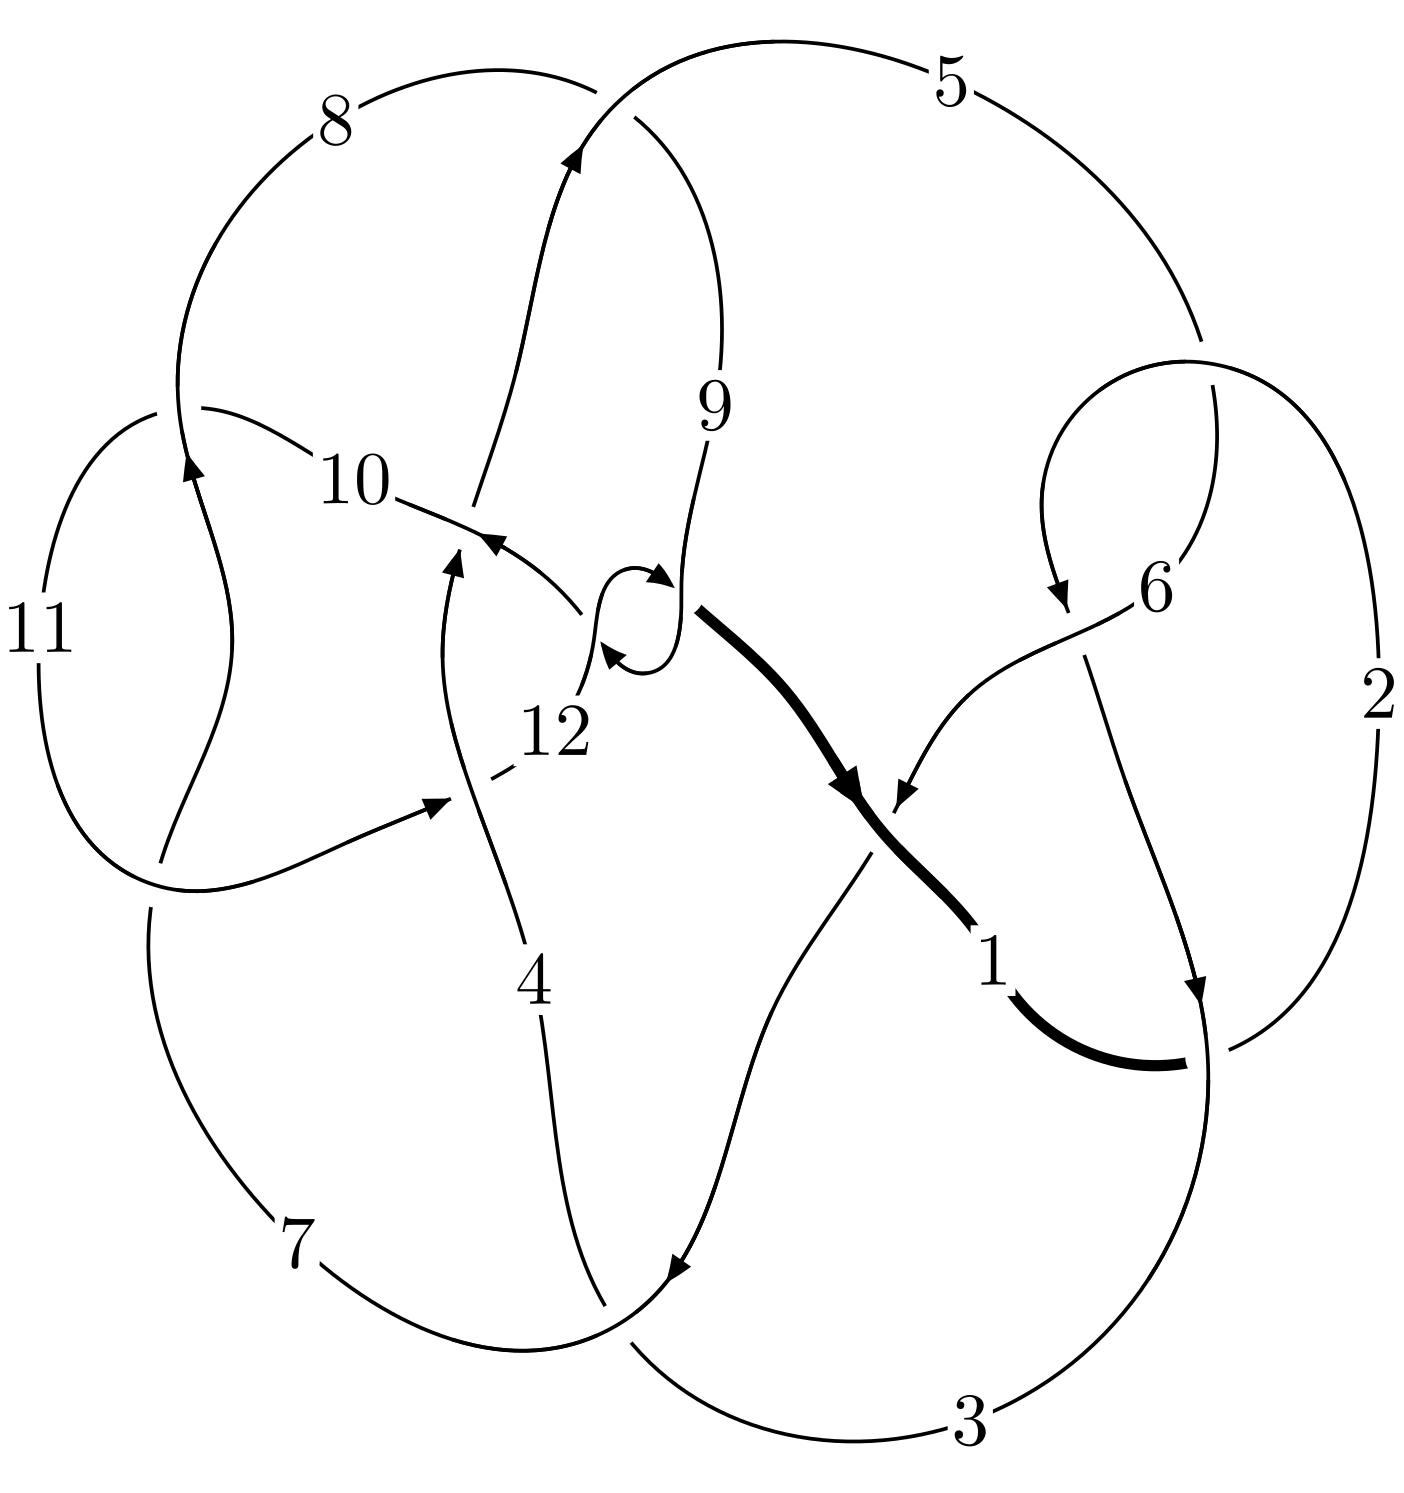
\includegraphics[width=112pt]{../../../GIT/diagram.site/Diagrams/png/1046_12a_0245.png}\\
\ \ \ A knot diagram\footnotemark}&
\allowdisplaybreaks
\textbf{Linearized knot diagam} \\
\cline{2-2}
 &
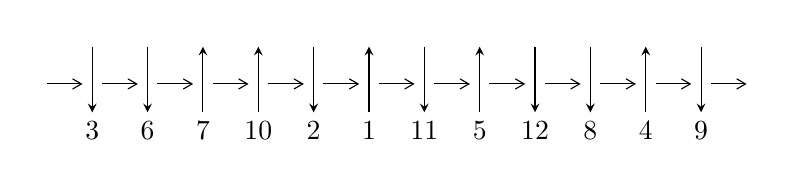
\begin{tikzpicture}[x=20pt, y=17pt]
	% nodes
	\node (C0) at (0, 0) {};
	\node (C1) at (1, 0) {};
	\node (C1U) at (1, +1) {};
	\node (C1D) at (1, -1) {3};

	\node (C2) at (2, 0) {};
	\node (C2U) at (2, +1) {};
	\node (C2D) at (2, -1) {6};

	\node (C3) at (3, 0) {};
	\node (C3U) at (3, +1) {};
	\node (C3D) at (3, -1) {7};

	\node (C4) at (4, 0) {};
	\node (C4U) at (4, +1) {};
	\node (C4D) at (4, -1) {10};

	\node (C5) at (5, 0) {};
	\node (C5U) at (5, +1) {};
	\node (C5D) at (5, -1) {2};

	\node (C6) at (6, 0) {};
	\node (C6U) at (6, +1) {};
	\node (C6D) at (6, -1) {1};

	\node (C7) at (7, 0) {};
	\node (C7U) at (7, +1) {};
	\node (C7D) at (7, -1) {11};

	\node (C8) at (8, 0) {};
	\node (C8U) at (8, +1) {};
	\node (C8D) at (8, -1) {5};

	\node (C9) at (9, 0) {};
	\node (C9U) at (9, +1) {};
	\node (C9D) at (9, -1) {12};

	\node (C10) at (10, 0) {};
	\node (C10U) at (10, +1) {};
	\node (C10D) at (10, -1) {8};

	\node (C11) at (11, 0) {};
	\node (C11U) at (11, +1) {};
	\node (C11D) at (11, -1) {4};

	\node (C12) at (12, 0) {};
	\node (C12U) at (12, +1) {};
	\node (C12D) at (12, -1) {9};
	\node (C13) at (13, 0) {};

	% arrows
	\draw[->,>={angle 60}]
	(C0) edge (C1) (C1) edge (C2) (C2) edge (C3) (C3) edge (C4) (C4) edge (C5) (C5) edge (C6) (C6) edge (C7) (C7) edge (C8) (C8) edge (C9) (C9) edge (C10) (C10) edge (C11) (C11) edge (C12) (C12) edge (C13) ;	\draw[->,>=stealth]
	(C1U) edge (C1D) (C2U) edge (C2D) (C3D) edge (C3U) (C4D) edge (C4U) (C5U) edge (C5D) (C6D) edge (C6U) (C7U) edge (C7D) (C8D) edge (C8U) (C9U) edge (C9D) (C10U) edge (C10D) (C11D) edge (C11U) (C12U) edge (C12D) ;
	\end{tikzpicture} \\
\hhline{~~} \\& 
\textbf{Solving Sequence} \\ \cline{2-2} 
 &
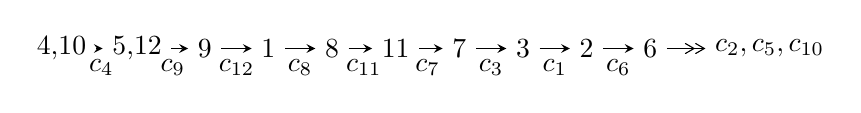
\begin{tikzpicture}[x=23pt, y=7pt]
	% node
	\node (A0) at (-1/8, 0) {4,10};
	\node (A1) at (17/16, 0) {5,12};
	\node (A2) at (17/8, 0) {9};
	\node (A3) at (25/8, 0) {1};
	\node (A4) at (33/8, 0) {8};
	\node (A5) at (41/8, 0) {11};
	\node (A6) at (49/8, 0) {7};
	\node (A7) at (57/8, 0) {3};
	\node (A8) at (65/8, 0) {2};
	\node (A9) at (73/8, 0) {6};
	\node (C1) at (1/2, -1) {$c_{4}$};
	\node (C2) at (13/8, -1) {$c_{9}$};
	\node (C3) at (21/8, -1) {$c_{12}$};
	\node (C4) at (29/8, -1) {$c_{8}$};
	\node (C5) at (37/8, -1) {$c_{11}$};
	\node (C6) at (45/8, -1) {$c_{7}$};
	\node (C7) at (53/8, -1) {$c_{3}$};
	\node (C8) at (61/8, -1) {$c_{1}$};
	\node (C9) at (69/8, -1) {$c_{6}$};
	\node (A10) at (11, 0) {$c_{2},c_{5},c_{10}$};

	% edge
	\draw[->,>=stealth]	
	(A0) edge (A1) (A1) edge (A2) (A2) edge (A3) (A3) edge (A4) (A4) edge (A5) (A5) edge (A6) (A6) edge (A7) (A7) edge (A8) (A8) edge (A9) ;
	\draw[->>,>={angle 60}]	
	(A9) edge (A10);
\end{tikzpicture} \\ 

\end{tabular} \\

\footnotetext{
The image of knot diagram is generated by the software ``\textbf{Draw programme}" developed by Andrew Bartholomew(\url{http://www.layer8.co.uk/maths/draw/index.htm\#Running-draw}), where we modified some parts for our purpose(\url{https://github.com/CATsTAILs/LinksPainter}).
}\phantom \\ \newline 
\centering \textbf{Ideals for irreducible components\footnotemark of $X_{\text{par}}$} 
 
\begin{align*}
I^u_{1}&=\langle 
-1.30829\times10^{182} u^{45}+3.21690\times10^{182} u^{44}+\cdots+2.91664\times10^{185} b+1.81261\times10^{186},\\
\phantom{I^u_{1}}&\phantom{= \langle  }2.74927\times10^{182} u^{45}-1.01973\times10^{183} u^{44}+\cdots+5.83327\times10^{185} a-1.27181\times10^{187},\\
\phantom{I^u_{1}}&\phantom{= \langle  }u^{46}-3 u^{45}+\cdots-30720 u+8192\rangle \\
I^u_{2}&=\langle 
- u^{31}- u^{30}+\cdots- a-2,\;2 u^{31}+u^{30}+\cdots+a^2+3,\;u^{32}+u^{31}+\cdots+2 u+1\rangle \\
I^u_{3}&=\langle 
u^2 a- u^3- u^2+b- a,\;a^2- a u- u,\;u^4+u^3+1\rangle \\
I^u_{4}&=\langle 
b+1,\;a^2- a+2,\;u-1\rangle \\
I^u_{5}&=\langle 
b- u-1,\;a-1,\;u^2+1\rangle \\
\\
I^v_{1}&=\langle 
a,\;v^5+2 v^4-16 v^2+64 b-16 v+32,\;v^6+2 v^5-16 v^3-16 v^2+32 v+64\rangle \\
\end{align*}
\raggedright * 6 irreducible components of $\dim_{\mathbb{C}}=0$, with total 128 representations.\\
\footnotetext{All coefficients of polynomials are rational numbers. But the coefficients are sometimes approximated in decimal forms when there is not enough margin.}
\newpage
\renewcommand{\arraystretch}{1}
\centering \section*{I. $I^u_{1}= \langle -1.31\times10^{182} u^{45}+3.22\times10^{182} u^{44}+\cdots+2.92\times10^{185} b+1.81\times10^{186},\;2.75\times10^{182} u^{45}-1.02\times10^{183} u^{44}+\cdots+5.83\times10^{185} a-1.27\times10^{187},\;u^{46}-3 u^{45}+\cdots-30720 u+8192 \rangle$}
\flushleft \textbf{(i) Arc colorings}\\
\begin{tabular}{m{7pt} m{180pt} m{7pt} m{180pt} }
\flushright $a_{4}=$&$\begin{pmatrix}1\\0\end{pmatrix}$ \\
\flushright $a_{10}=$&$\begin{pmatrix}0\\u\end{pmatrix}$ \\
\flushright $a_{5}=$&$\begin{pmatrix}1\\- u^2\end{pmatrix}$ \\
\flushright $a_{12}=$&$\begin{pmatrix}-0.000471309 u^{45}+0.00174813 u^{44}+\cdots-24.9228 u+21.8026\\0.000448560 u^{45}-0.00110295 u^{44}+\cdots+13.9436 u-6.21474\end{pmatrix}$ \\
\flushright $a_{9}=$&$\begin{pmatrix}0.000919870 u^{45}-0.00285108 u^{44}+\cdots+38.8664 u-28.0174\\0.000859527 u^{45}-0.00194940 u^{44}+\cdots+24.2892 u-6.96411\end{pmatrix}$ \\
\flushright $a_{1}=$&$\begin{pmatrix}-0.000531652 u^{45}+0.00264982 u^{44}+\cdots-40.4999 u+42.8559\\0.000478275 u^{45}-0.00119240 u^{44}+\cdots+14.5999 u-7.27524\end{pmatrix}$ \\
\flushright $a_{8}=$&$\begin{pmatrix}0.000471309 u^{45}-0.00174813 u^{44}+\cdots+24.9228 u-21.8026\\0.000991814 u^{45}-0.00227861 u^{44}+\cdots+28.0713 u-8.95256\end{pmatrix}$ \\
\flushright $a_{11}=$&$\begin{pmatrix}-0.000919870 u^{45}+0.00285108 u^{44}+\cdots-38.8664 u+28.0174\\0.000448560 u^{45}-0.00110295 u^{44}+\cdots+13.9436 u-6.21474\end{pmatrix}$ \\
\flushright $a_{7}=$&$\begin{pmatrix}0.000531652 u^{45}-0.00264982 u^{44}+\cdots+40.4999 u-42.8559\\0.00185134 u^{45}-0.00422801 u^{44}+\cdots+51.3606 u-15.9167\end{pmatrix}$ \\
\flushright $a_{3}=$&$\begin{pmatrix}0.00115169 u^{45}-0.00185933 u^{44}+\cdots+29.6103 u+9.69006\\0.00179201 u^{45}-0.00442512 u^{44}+\cdots+55.3750 u-28.2489\end{pmatrix}$ \\
\flushright $a_{2}=$&$\begin{pmatrix}-0.000177162 u^{45}+0.00141815 u^{44}+\cdots-33.1849 u+22.5187\\0.000323331 u^{45}-0.00109532 u^{44}+\cdots+8.96510 u-11.5651\end{pmatrix}$ \\
\flushright $a_{6}=$&$\begin{pmatrix}0.00269326 u^{45}-0.00782283 u^{44}+\cdots+106.019 u-66.8639\\-0.00167414 u^{45}+0.00452784 u^{44}+\cdots-49.4479 u+36.0030\end{pmatrix}$\\&\end{tabular}
\flushleft \textbf{(ii) Obstruction class $= -1$}\\~\\
\flushleft \textbf{(iii) Cusp Shapes $= 0.000526625 u^{45}-0.00139921 u^{44}+\cdots+30.9656 u+16.8615$}\\~\\
\newpage\renewcommand{\arraystretch}{1}
\flushleft \textbf{(iv) u-Polynomials at the component}\newline \\
\begin{tabular}{m{50pt}|m{274pt}}
Crossings & \hspace{64pt}u-Polynomials at each crossing \\
\hline $$\begin{aligned}c_{1}\end{aligned}$$&$\begin{aligned}
&u^{46}+22 u^{45}+\cdots+65 u+16
\end{aligned}$\\
\hline $$\begin{aligned}c_{2},c_{5}\end{aligned}$$&$\begin{aligned}
&u^{46}+2 u^{45}+\cdots+15 u+4
\end{aligned}$\\
\hline $$\begin{aligned}c_{3}\end{aligned}$$&$\begin{aligned}
&u^{46}+2 u^{45}+\cdots+419884 u+136336
\end{aligned}$\\
\hline $$\begin{aligned}c_{4}\end{aligned}$$&$\begin{aligned}
&u^{46}+3 u^{45}+\cdots+30720 u+8192
\end{aligned}$\\
\hline $$\begin{aligned}c_{6}\end{aligned}$$&$\begin{aligned}
&u^{46}+2 u^{44}+\cdots+2032 u+448
\end{aligned}$\\
\hline $$\begin{aligned}c_{7},c_{9},c_{10}\\c_{12}\end{aligned}$$&$\begin{aligned}
&u^{46}+6 u^{45}+\cdots-6 u+1
\end{aligned}$\\
\hline $$\begin{aligned}c_{8},c_{11}\end{aligned}$$&$\begin{aligned}
&64(64 u^{46}-96 u^{45}+\cdots-8 u^2+2)
\end{aligned}$\\
\hline
\end{tabular}\\~\\
\newpage\renewcommand{\arraystretch}{1}
\flushleft \textbf{(v) Riley Polynomials at the component}\newline \\
\begin{tabular}{m{50pt}|m{274pt}}
Crossings & \hspace{64pt}Riley Polynomials at each crossing \\
\hline $$\begin{aligned}c_{1}\end{aligned}$$&$\begin{aligned}
&y^{46}+6 y^{45}+\cdots+3391 y+256
\end{aligned}$\\
\hline $$\begin{aligned}c_{2},c_{5}\end{aligned}$$&$\begin{aligned}
&y^{46}-22 y^{45}+\cdots-65 y+16
\end{aligned}$\\
\hline $$\begin{aligned}c_{3}\end{aligned}$$&$\begin{aligned}
&y^{46}-30 y^{45}+\cdots-205613722768 y+18587504896
\end{aligned}$\\
\hline $$\begin{aligned}c_{4}\end{aligned}$$&$\begin{aligned}
&y^{46}-11 y^{45}+\cdots-1572864000 y+67108864
\end{aligned}$\\
\hline $$\begin{aligned}c_{6}\end{aligned}$$&$\begin{aligned}
&y^{46}+4 y^{45}+\cdots+910080 y+200704
\end{aligned}$\\
\hline $$\begin{aligned}c_{7},c_{9},c_{10}\\c_{12}\end{aligned}$$&$\begin{aligned}
&y^{46}+26 y^{45}+\cdots-12 y+1
\end{aligned}$\\
\hline $$\begin{aligned}c_{8},c_{11}\end{aligned}$$&$\begin{aligned}
&4096(4096 y^{46}-93184 y^{45}+\cdots-32 y+4)
\end{aligned}$\\
\hline
\end{tabular}\\~\\
\newpage\flushleft \textbf{(vi) Complex Volumes and Cusp Shapes}
$$\begin{array}{c|c|c}  
\text{Solutions to }I^u_{1}& \I (\text{vol} + \sqrt{-1}CS) & \text{Cusp shape}\\
 \hline 
\begin{aligned}
u &= -0.401792 + 0.789673 I \\
a &= \phantom{-}1.034950 + 0.489117 I \\
b &= -0.098777 + 0.739250 I\end{aligned}
 & -3.37451 + 5.47103 I & -6.94202 - 5.47084 I \\ \hline\begin{aligned}
u &= -0.401792 - 0.789673 I \\
a &= \phantom{-}1.034950 - 0.489117 I \\
b &= -0.098777 - 0.739250 I\end{aligned}
 & -3.37451 - 5.47103 I & -6.94202 + 5.47084 I \\ \hline\begin{aligned}
u &= \phantom{-}0.239618 + 0.727911 I \\
a &= -0.877973 + 0.679500 I \\
b &= \phantom{-}0.064614 + 0.618606 I\end{aligned}
 & -1.23789 - 1.34787 I & -5.39091 + 2.19254 I \\ \hline\begin{aligned}
u &= \phantom{-}0.239618 - 0.727911 I \\
a &= -0.877973 - 0.679500 I \\
b &= \phantom{-}0.064614 - 0.618606 I\end{aligned}
 & -1.23789 + 1.34787 I & -5.39091 - 2.19254 I \\ \hline\begin{aligned}
u &= -0.078679 + 0.719346 I \\
a &= -0.451493 + 0.580682 I \\
b &= -0.063814 + 0.526016 I\end{aligned}
 & -0.697121 - 1.212220 I & -4.01044 + 6.14816 I \\ \hline\begin{aligned}
u &= -0.078679 - 0.719346 I \\
a &= -0.451493 - 0.580682 I \\
b &= -0.063814 - 0.526016 I\end{aligned}
 & -0.697121 + 1.212220 I & -4.01044 - 6.14816 I \\ \hline\begin{aligned}
u &= -0.433643 + 0.566016 I \\
a &= \phantom{-}1.33364 + 0.69018 I \\
b &= -0.273046 + 0.628978 I\end{aligned}
 & -4.26962 - 1.33304 I & -9.23410 + 6.58879 I \\ \hline\begin{aligned}
u &= -0.433643 - 0.566016 I \\
a &= \phantom{-}1.33364 - 0.69018 I \\
b &= -0.273046 - 0.628978 I\end{aligned}
 & -4.26962 + 1.33304 I & -9.23410 - 6.58879 I \\ \hline\begin{aligned}
u &= \phantom{-}0.672328 + 0.122077 I \\
a &= -2.03352 + 0.16905 I \\
b &= \phantom{-}0.811410 + 0.208117 I\end{aligned}
 & -1.01846 + 6.05975 I & \phantom{-}5.32943 - 7.91016 I \\ \hline\begin{aligned}
u &= \phantom{-}0.672328 - 0.122077 I \\
a &= -2.03352 - 0.16905 I \\
b &= \phantom{-}0.811410 - 0.208117 I\end{aligned}
 & -1.01846 - 6.05975 I & \phantom{-}5.32943 + 7.91016 I\\
 \hline 
 \end{array}$$\newpage$$\begin{array}{c|c|c}  
\text{Solutions to }I^u_{1}& \I (\text{vol} + \sqrt{-1}CS) & \text{Cusp shape}\\
 \hline 
\begin{aligned}
u &= -0.645073 + 0.070271 I \\
a &= \phantom{-}2.10420 + 0.11324 I \\
b &= -0.777175 + 0.116055 I\end{aligned}
 & \phantom{-}0.827180 - 1.119400 I & \phantom{-}9.81417 + 2.37316 I \\ \hline\begin{aligned}
u &= -0.645073 - 0.070271 I \\
a &= \phantom{-}2.10420 - 0.11324 I \\
b &= -0.777175 - 0.116055 I\end{aligned}
 & \phantom{-}0.827180 + 1.119400 I & \phantom{-}9.81417 - 2.37316 I \\ \hline\begin{aligned}
u &= \phantom{-}0.520537 + 0.295551 I \\
a &= \phantom{-}0.413738 + 0.318781 I \\
b &= \phantom{-}0.371984 + 0.476647 I\end{aligned}
 & -1.97267 - 1.37276 I & -2.57483 + 1.51766 I \\ \hline\begin{aligned}
u &= \phantom{-}0.520537 - 0.295551 I \\
a &= \phantom{-}0.413738 - 0.318781 I \\
b &= \phantom{-}0.371984 - 0.476647 I\end{aligned}
 & -1.97267 + 1.37276 I & -2.57483 - 1.51766 I \\ \hline\begin{aligned}
u &= \phantom{-}0.502594 + 0.228503 I \\
a &= -2.11877 + 0.56848 I \\
b &= \phantom{-}0.525503 + 0.309703 I\end{aligned}
 & -3.39297 - 0.50689 I & \phantom{-}1.54331 - 8.55618 I \\ \hline\begin{aligned}
u &= \phantom{-}0.502594 - 0.228503 I \\
a &= -2.11877 - 0.56848 I \\
b &= \phantom{-}0.525503 - 0.309703 I\end{aligned}
 & -3.39297 + 0.50689 I & \phantom{-}1.54331 + 8.55618 I \\ \hline\begin{aligned}
u &= \phantom{-}0.532699 + 0.084051 I \\
a &= \phantom{-}0.573143 + 0.199439 I \\
b &= \phantom{-}0.707726 + 0.345489 I\end{aligned}
 & -0.46138 + 5.41462 I & \phantom{-}2.43162 - 4.62417 I \\ \hline\begin{aligned}
u &= \phantom{-}0.532699 - 0.084051 I \\
a &= \phantom{-}0.573143 - 0.199439 I \\
b &= \phantom{-}0.707726 - 0.345489 I\end{aligned}
 & -0.46138 - 5.41462 I & \phantom{-}2.43162 + 4.62417 I \\ \hline\begin{aligned}
u &= -0.478597 + 0.061203 I \\
a &= -0.523519 + 0.112067 I \\
b &= -0.641497 + 0.184230 I\end{aligned}
 & \phantom{-}1.49547 - 0.77471 I & \phantom{-}6.52139 + 0.61017 I \\ \hline\begin{aligned}
u &= -0.478597 - 0.061203 I \\
a &= -0.523519 - 0.112067 I \\
b &= -0.641497 - 0.184230 I\end{aligned}
 & \phantom{-}1.49547 + 0.77471 I & \phantom{-}6.52139 - 0.61017 I\\
 \hline 
 \end{array}$$\newpage$$\begin{array}{c|c|c}  
\text{Solutions to }I^u_{1}& \I (\text{vol} + \sqrt{-1}CS) & \text{Cusp shape}\\
 \hline 
\begin{aligned}
u &= \phantom{-}1.32298 + 1.00419 I \\
a &= -0.244934 - 0.868893 I \\
b &= -1.59181 - 1.00368 I\end{aligned}
 & \phantom{-}7.9562 + 18.9510 I & \phantom{-0.000000 } 0 \\ \hline\begin{aligned}
u &= \phantom{-}1.32298 - 1.00419 I \\
a &= -0.244934 + 0.868893 I \\
b &= -1.59181 + 1.00368 I\end{aligned}
 & \phantom{-}7.9562 - 18.9510 I & \phantom{-0.000000 } 0 \\ \hline\begin{aligned}
u &= \phantom{-}1.36201 + 0.97857 I \\
a &= -0.221655 - 0.833836 I \\
b &= -1.46345 - 0.96268 I\end{aligned}
 & \phantom{-}4.87739 + 11.08340 I & \phantom{-0.000000 } 0 \\ \hline\begin{aligned}
u &= \phantom{-}1.36201 - 0.97857 I \\
a &= -0.221655 + 0.833836 I \\
b &= -1.46345 + 0.96268 I\end{aligned}
 & \phantom{-}4.87739 - 11.08340 I & \phantom{-0.000000 } 0 \\ \hline\begin{aligned}
u &= -1.33866 + 1.01035 I \\
a &= \phantom{-}0.250581 - 0.854142 I \\
b &= \phantom{-}1.57565 - 0.95478 I\end{aligned}
 & \phantom{-}10.1320 - 13.6218 I & \phantom{-0.000000 } 0 \\ \hline\begin{aligned}
u &= -1.33866 - 1.01035 I \\
a &= \phantom{-}0.250581 + 0.854142 I \\
b &= \phantom{-}1.57565 + 0.95478 I\end{aligned}
 & \phantom{-}10.1320 + 13.6218 I & \phantom{-0.000000 } 0 \\ \hline\begin{aligned}
u &= -1.38555 + 1.03866 I \\
a &= \phantom{-}0.272974 - 0.808895 I \\
b &= \phantom{-}1.53500 - 0.79923 I\end{aligned}
 & \phantom{-}11.2953 - 10.4811 I & \phantom{-0.000000 } 0 \\ \hline\begin{aligned}
u &= -1.38555 - 1.03866 I \\
a &= \phantom{-}0.272974 + 0.808895 I \\
b &= \phantom{-}1.53500 + 0.79923 I\end{aligned}
 & \phantom{-}11.2953 + 10.4811 I & \phantom{-0.000000 } 0 \\ \hline\begin{aligned}
u &= -1.57230 + 0.77246 I \\
a &= \phantom{-}0.085159 - 0.690200 I \\
b &= \phantom{-}0.913569 - 0.867748 I\end{aligned}
 & \phantom{-}0.59144 - 10.81880 I & \phantom{-0.000000 } 0 \\ \hline\begin{aligned}
u &= -1.57230 - 0.77246 I \\
a &= \phantom{-}0.085159 + 0.690200 I \\
b &= \phantom{-}0.913569 + 0.867748 I\end{aligned}
 & \phantom{-}0.59144 + 10.81880 I & \phantom{-0.000000 } 0\\
 \hline 
 \end{array}$$\newpage$$\begin{array}{c|c|c}  
\text{Solutions to }I^u_{1}& \I (\text{vol} + \sqrt{-1}CS) & \text{Cusp shape}\\
 \hline 
\begin{aligned}
u &= \phantom{-}1.41374 + 1.05421 I \\
a &= -0.282174 - 0.781521 I \\
b &= -1.49805 - 0.71794 I\end{aligned}
 & \phantom{-}10.12260 + 5.12502 I & \phantom{-0.000000 } 0 \\ \hline\begin{aligned}
u &= \phantom{-}1.41374 - 1.05421 I \\
a &= -0.282174 + 0.781521 I \\
b &= -1.49805 + 0.71794 I\end{aligned}
 & \phantom{-}10.12260 - 5.12502 I & \phantom{-0.000000 } 0 \\ \hline\begin{aligned}
u &= \phantom{-}1.69696 + 0.85231 I \\
a &= -0.124053 - 0.627843 I \\
b &= -0.899624 - 0.686359 I\end{aligned}
 & \phantom{-}3.79825 + 6.24987 I & \phantom{-0.000000 } 0 \\ \hline\begin{aligned}
u &= \phantom{-}1.69696 - 0.85231 I \\
a &= -0.124053 + 0.627843 I \\
b &= -0.899624 + 0.686359 I\end{aligned}
 & \phantom{-}3.79825 - 6.24987 I & \phantom{-0.000000 } 0 \\ \hline\begin{aligned}
u &= -1.88174 + 0.67526 I \\
a &= \phantom{-}0.052037 - 0.556937 I \\
b &= \phantom{-}0.669760 - 0.655489 I\end{aligned}
 & -0.19317 - 2.26026 I & \phantom{-0.000000 } 0 \\ \hline\begin{aligned}
u &= -1.88174 - 0.67526 I \\
a &= \phantom{-}0.052037 + 0.556937 I \\
b &= \phantom{-}0.669760 + 0.655489 I\end{aligned}
 & -0.19317 + 2.26026 I & \phantom{-0.000000 } 0 \\ \hline\begin{aligned}
u &= \phantom{-}1.15493 + 1.84484 I \\
a &= -0.522503 - 0.223781 I \\
b &= -0.696453 + 0.457576 I\end{aligned}
 & \phantom{-}6.20944 - 9.54624 I & \phantom{-0.000000 } 0 \\ \hline\begin{aligned}
u &= \phantom{-}1.15493 - 1.84484 I \\
a &= -0.522503 + 0.223781 I \\
b &= -0.696453 - 0.457576 I\end{aligned}
 & \phantom{-}6.20944 + 9.54624 I & \phantom{-0.000000 } 0 \\ \hline\begin{aligned}
u &= \phantom{-}1.71157 + 1.45820 I \\
a &= -0.345297 - 0.457141 I \\
b &= -0.959259 - 0.047672 I\end{aligned}
 & \phantom{-}9.03151 + 5.36539 I & \phantom{-0.000000 } 0 \\ \hline\begin{aligned}
u &= \phantom{-}1.71157 - 1.45820 I \\
a &= -0.345297 + 0.457141 I \\
b &= -0.959259 + 0.047672 I\end{aligned}
 & \phantom{-}9.03151 - 5.36539 I & \phantom{-0.000000 } 0\\
 \hline 
 \end{array}$$\newpage$$\begin{array}{c|c|c}  
\text{Solutions to }I^u_{1}& \I (\text{vol} + \sqrt{-1}CS) & \text{Cusp shape}\\
 \hline 
\begin{aligned}
u &= -1.29479 + 1.87645 I \\
a &= \phantom{-}0.478230 - 0.255335 I \\
b &= \phantom{-}0.724784 + 0.367690 I\end{aligned}
 & \phantom{-}8.41076 + 3.99047 I & \phantom{-0.000000 } 0 \\ \hline\begin{aligned}
u &= -1.29479 - 1.87645 I \\
a &= \phantom{-}0.478230 + 0.255335 I \\
b &= \phantom{-}0.724784 - 0.367690 I\end{aligned}
 & \phantom{-}8.41076 - 3.99047 I & \phantom{-0.000000 } 0 \\ \hline\begin{aligned}
u &= -1.65453 + 1.63052 I \\
a &= \phantom{-}0.382255 - 0.391673 I \\
b &= \phantom{-}0.882553 + 0.091874 I\end{aligned}
 & \phantom{-}9.95002 + 0.24033 I & \phantom{-0.000000 } 0 \\ \hline\begin{aligned}
u &= -1.65453 - 1.63052 I \\
a &= \phantom{-}0.382255 + 0.391673 I \\
b &= \phantom{-}0.882553 - 0.091874 I\end{aligned}
 & \phantom{-}9.95002 - 0.24033 I & \phantom{-0.000000 } 0 \\ \hline\begin{aligned}
u &= \phantom{-}1.53540 + 2.28777 I \\
a &= -0.360009 - 0.207800 I \\
b &= -0.569607 + 0.219649 I\end{aligned}
 & \phantom{-}2.65240 - 1.11142 I & \phantom{-0.000000 } 0 \\ \hline\begin{aligned}
u &= \phantom{-}1.53540 - 2.28777 I \\
a &= -0.360009 + 0.207800 I \\
b &= -0.569607 - 0.219649 I\end{aligned}
 & \phantom{-}2.65240 + 1.11142 I & \phantom{-0.000000 } 0\\
 \hline 
 \end{array}$$\newpage\newpage\renewcommand{\arraystretch}{1}
\centering \section*{II. $I^u_{2}= \langle - u^{31}- u^{30}+\cdots- a-2,\;2 u^{31}+u^{30}+\cdots+a^2+3,\;u^{32}+u^{31}+\cdots+2 u+1 \rangle$}
\flushleft \textbf{(i) Arc colorings}\\
\begin{tabular}{m{7pt} m{180pt} m{7pt} m{180pt} }
\flushright $a_{4}=$&$\begin{pmatrix}1\\0\end{pmatrix}$ \\
\flushright $a_{10}=$&$\begin{pmatrix}0\\u\end{pmatrix}$ \\
\flushright $a_{5}=$&$\begin{pmatrix}1\\- u^2\end{pmatrix}$ \\
\flushright $a_{12}=$&$\begin{pmatrix}a\\u^{31}+u^{30}+\cdots+a+2\end{pmatrix}$ \\
\flushright $a_{9}=$&$\begin{pmatrix}u^{31}+u^{30}+\cdots+u+2\\u^{31}+u^{30}+\cdots- a+2\end{pmatrix}$ \\
\flushright $a_{1}=$&$\begin{pmatrix}- u^5- u\\u^7- u^5+2 u^3- u\end{pmatrix}$ \\
\flushright $a_{8}=$&$\begin{pmatrix}a- u\\u^{31}+u^{30}+\cdots- a+2\end{pmatrix}$ \\
\flushright $a_{11}=$&$\begin{pmatrix}- u^{31}- u^{30}+\cdots- u-2\\u^{31}+u^{30}+\cdots+a+2\end{pmatrix}$ \\
\flushright $a_{7}=$&$\begin{pmatrix}u^5+u\\- u^5+u^3- u\end{pmatrix}$ \\
\flushright $a_{3}=$&$\begin{pmatrix}- u^{10}+u^8-2 u^6+u^4- u^2+1\\u^{10}-2 u^8+3 u^6-2 u^4+u^2\end{pmatrix}$ \\
\flushright $a_{2}=$&$\begin{pmatrix}- u^{27}+4 u^{25}+\cdots+10 u^5-5 u^3\\u^{27}-5 u^{25}+\cdots+3 u^3- u\end{pmatrix}$ \\
\flushright $a_{6}=$&$\begin{pmatrix}- u^{17}+2 u^{15}-5 u^{13}+6 u^{11}-7 u^9+6 u^7-2 u^5+2 u^3+u\\u^{19}-3 u^{17}+8 u^{15}-13 u^{13}+17 u^{11}-17 u^9+12 u^7-8 u^5+3 u^3- u\end{pmatrix}$\\&\end{tabular}
\flushleft \textbf{(ii) Obstruction class $= -1$}\\~\\
\flushleft \textbf{(iii) Cusp Shapes $= -4 u^{30}+20 u^{28}+4 u^{27}-68 u^{26}-20 u^{25}+156 u^{24}+68 u^{23}-276 u^{22}-160 u^{21}+380 u^{20}+292 u^{19}-404 u^{18}-428 u^{17}+328 u^{16}+504 u^{15}-160 u^{14}-496 u^{13}-8 u^{12}+392 u^{11}+124 u^{10}-252 u^9-156 u^8+120 u^7+116 u^6-28 u^5-64 u^4-4 u^3+16 u^2+12 u-2$}\\~\\
\newpage\renewcommand{\arraystretch}{1}
\flushleft \textbf{(iv) u-Polynomials at the component}\newline \\
\begin{tabular}{m{50pt}|m{274pt}}
Crossings & \hspace{64pt}u-Polynomials at each crossing \\
\hline $$\begin{aligned}c_{1}\end{aligned}$$&$\begin{aligned}
&(u^{32}+15 u^{31}+\cdots+2 u+1)^{2}
\end{aligned}$\\
\hline $$\begin{aligned}c_{2},c_{5}\end{aligned}$$&$\begin{aligned}
&(u^{32}+u^{31}+\cdots- u^2+1)^{2}
\end{aligned}$\\
\hline $$\begin{aligned}c_{3}\end{aligned}$$&$\begin{aligned}
&(u^{32}+4 u^{31}+\cdots+28 u+4)^{2}
\end{aligned}$\\
\hline $$\begin{aligned}c_{4}\end{aligned}$$&$\begin{aligned}
&(u^{32}- u^{31}+\cdots-2 u+1)^{2}
\end{aligned}$\\
\hline $$\begin{aligned}c_{6}\end{aligned}$$&$\begin{aligned}
&(u^{32}+3 u^{31}+\cdots+2 u+3)^{2}
\end{aligned}$\\
\hline $$\begin{aligned}c_{7},c_{9},c_{10}\\c_{12}\end{aligned}$$&$\begin{aligned}
&u^{64}-11 u^{63}+\cdots+4 u+1
\end{aligned}$\\
\hline $$\begin{aligned}c_{8},c_{11}\end{aligned}$$&$\begin{aligned}
&u^{64}+u^{63}+\cdots-8574468 u+1426351
\end{aligned}$\\
\hline
\end{tabular}\\~\\
\newpage\renewcommand{\arraystretch}{1}
\flushleft \textbf{(v) Riley Polynomials at the component}\newline \\
\begin{tabular}{m{50pt}|m{274pt}}
Crossings & \hspace{64pt}Riley Polynomials at each crossing \\
\hline $$\begin{aligned}c_{1}\end{aligned}$$&$\begin{aligned}
&(y^{32}+5 y^{31}+\cdots+2 y+1)^{2}
\end{aligned}$\\
\hline $$\begin{aligned}c_{2},c_{5}\end{aligned}$$&$\begin{aligned}
&(y^{32}-15 y^{31}+\cdots-2 y+1)^{2}
\end{aligned}$\\
\hline $$\begin{aligned}c_{3}\end{aligned}$$&$\begin{aligned}
&(y^{32}-20 y^{31}+\cdots-184 y+16)^{2}
\end{aligned}$\\
\hline $$\begin{aligned}c_{4}\end{aligned}$$&$\begin{aligned}
&(y^{32}-11 y^{31}+\cdots-2 y+1)^{2}
\end{aligned}$\\
\hline $$\begin{aligned}c_{6}\end{aligned}$$&$\begin{aligned}
&(y^{32}+5 y^{31}+\cdots+164 y+9)^{2}
\end{aligned}$\\
\hline $$\begin{aligned}c_{7},c_{9},c_{10}\\c_{12}\end{aligned}$$&$\begin{aligned}
&y^{64}+43 y^{63}+\cdots-58 y+1
\end{aligned}$\\
\hline $$\begin{aligned}c_{8},c_{11}\end{aligned}$$&$\begin{aligned}
&y^{64}-33 y^{63}+\cdots-47292589687204 y+2034477175201
\end{aligned}$\\
\hline
\end{tabular}\\~\\
\newpage\flushleft \textbf{(vi) Complex Volumes and Cusp Shapes}
$$\begin{array}{c|c|c}  
\text{Solutions to }I^u_{2}& \I (\text{vol} + \sqrt{-1}CS) & \text{Cusp shape}\\
 \hline 
\begin{aligned}
u &= -0.613006 + 0.792175 I \\
a &= -0.991143 + 0.568727 I \\
b &= -1.182060 + 0.538855 I\end{aligned}
 & \phantom{-}2.22015 + 7.30693 I & -2.17644 - 4.86883 I \\ \hline\begin{aligned}
u &= -0.613006 + 0.792175 I \\
a &= \phantom{-}0.378138 + 0.223448 I \\
b &= \phantom{-}0.86730 + 1.43651 I\end{aligned}
 & \phantom{-}2.22015 + 7.30693 I & -2.17644 - 4.86883 I \\ \hline\begin{aligned}
u &= -0.613006 - 0.792175 I \\
a &= -0.991143 - 0.568727 I \\
b &= -1.182060 - 0.538855 I\end{aligned}
 & \phantom{-}2.22015 - 7.30693 I & -2.17644 + 4.86883 I \\ \hline\begin{aligned}
u &= -0.613006 - 0.792175 I \\
a &= \phantom{-}0.378138 - 0.223448 I \\
b &= \phantom{-}0.86730 - 1.43651 I\end{aligned}
 & \phantom{-}2.22015 - 7.30693 I & -2.17644 + 4.86883 I \\ \hline\begin{aligned}
u &= -0.674958 + 0.742403 I \\
a &= -0.814727 + 0.619700 I \\
b &= -0.843215 + 0.599874 I\end{aligned}
 & -0.345747 + 0.057794 I & -5.67435 + 0.61686 I \\ \hline\begin{aligned}
u &= -0.674958 + 0.742403 I \\
a &= \phantom{-}0.139769 + 0.122703 I \\
b &= \phantom{-}0.700606 + 1.011950 I\end{aligned}
 & -0.345747 + 0.057794 I & -5.67435 + 0.61686 I \\ \hline\begin{aligned}
u &= -0.674958 - 0.742403 I \\
a &= -0.814727 - 0.619700 I \\
b &= -0.843215 - 0.599874 I\end{aligned}
 & -0.345747 - 0.057794 I & -5.67435 - 0.61686 I \\ \hline\begin{aligned}
u &= -0.674958 - 0.742403 I \\
a &= \phantom{-}0.139769 - 0.122703 I \\
b &= \phantom{-}0.700606 - 1.011950 I\end{aligned}
 & -0.345747 - 0.057794 I & -5.67435 - 0.61686 I \\ \hline\begin{aligned}
u &= \phantom{-}0.600521 + 0.762759 I \\
a &= \phantom{-}0.990953 + 0.630677 I \\
b &= \phantom{-}1.150690 + 0.671706 I\end{aligned}
 & \phantom{-}4.27947 - 2.26361 I & \phantom{-}1.018945 + 0.670058 I \\ \hline\begin{aligned}
u &= \phantom{-}0.600521 + 0.762759 I \\
a &= -0.390433 + 0.132083 I \\
b &= -0.99299 + 1.32833 I\end{aligned}
 & \phantom{-}4.27947 - 2.26361 I & \phantom{-}1.018945 + 0.670058 I\\
 \hline 
 \end{array}$$\newpage$$\begin{array}{c|c|c}  
\text{Solutions to }I^u_{2}& \I (\text{vol} + \sqrt{-1}CS) & \text{Cusp shape}\\
 \hline 
\begin{aligned}
u &= \phantom{-}0.600521 - 0.762759 I \\
a &= \phantom{-}0.990953 - 0.630677 I \\
b &= \phantom{-}1.150690 - 0.671706 I\end{aligned}
 & \phantom{-}4.27947 + 2.26361 I & \phantom{-}1.018945 - 0.670058 I \\ \hline\begin{aligned}
u &= \phantom{-}0.600521 - 0.762759 I \\
a &= -0.390433 - 0.132083 I \\
b &= -0.99299 - 1.32833 I\end{aligned}
 & \phantom{-}4.27947 + 2.26361 I & \phantom{-}1.018945 - 0.670058 I \\ \hline\begin{aligned}
u &= -0.849583 + 0.407230 I \\
a &= -0.257323 - 0.869065 I \\
b &= \phantom{-}1.44423 - 0.10517 I\end{aligned}
 & \phantom{-}3.39887 - 4.15286 I & \phantom{-}2.01286 + 7.18864 I \\ \hline\begin{aligned}
u &= -0.849583 + 0.407230 I \\
a &= -0.592259 + 1.276300 I \\
b &= -0.188985 + 0.615704 I\end{aligned}
 & \phantom{-}3.39887 - 4.15286 I & \phantom{-}2.01286 + 7.18864 I \\ \hline\begin{aligned}
u &= -0.849583 - 0.407230 I \\
a &= -0.257323 + 0.869065 I \\
b &= \phantom{-}1.44423 + 0.10517 I\end{aligned}
 & \phantom{-}3.39887 + 4.15286 I & \phantom{-}2.01286 - 7.18864 I \\ \hline\begin{aligned}
u &= -0.849583 - 0.407230 I \\
a &= -0.592259 - 1.276300 I \\
b &= -0.188985 - 0.615704 I\end{aligned}
 & \phantom{-}3.39887 + 4.15286 I & \phantom{-}2.01286 - 7.18864 I \\ \hline\begin{aligned}
u &= -1.093530 + 0.032199 I \\
a &= -0.548154 - 1.299260 I \\
b &= \phantom{-}1.111940 + 0.241357 I\end{aligned}
 & \phantom{-}10.01990 - 1.36697 I & \phantom{-}7.90065 + 0.55023 I \\ \hline\begin{aligned}
u &= -1.093530 + 0.032199 I \\
a &= -0.54538 + 1.33146 I \\
b &= \phantom{-}0.926137 - 0.270830 I\end{aligned}
 & \phantom{-}10.01990 - 1.36697 I & \phantom{-}7.90065 + 0.55023 I \\ \hline\begin{aligned}
u &= -1.093530 - 0.032199 I \\
a &= -0.548154 + 1.299260 I \\
b &= \phantom{-}1.111940 - 0.241357 I\end{aligned}
 & \phantom{-}10.01990 + 1.36697 I & \phantom{-}7.90065 - 0.55023 I \\ \hline\begin{aligned}
u &= -1.093530 - 0.032199 I \\
a &= -0.54538 - 1.33146 I \\
b &= \phantom{-}0.926137 + 0.270830 I\end{aligned}
 & \phantom{-}10.01990 + 1.36697 I & \phantom{-}7.90065 - 0.55023 I\\
 \hline 
 \end{array}$$\newpage$$\begin{array}{c|c|c}  
\text{Solutions to }I^u_{2}& \I (\text{vol} + \sqrt{-1}CS) & \text{Cusp shape}\\
 \hline 
\begin{aligned}
u &= \phantom{-}1.098860 + 0.059621 I \\
a &= \phantom{-}0.552832 - 1.283140 I \\
b &= -1.188240 + 0.238476 I\end{aligned}
 & \phantom{-}8.24887 + 6.50568 I & \phantom{-}4.96918 - 5.51070 I \\ \hline\begin{aligned}
u &= \phantom{-}1.098860 + 0.059621 I \\
a &= \phantom{-}0.54603 + 1.34276 I \\
b &= -0.842777 - 0.296157 I\end{aligned}
 & \phantom{-}8.24887 + 6.50568 I & \phantom{-}4.96918 - 5.51070 I \\ \hline\begin{aligned}
u &= \phantom{-}1.098860 - 0.059621 I \\
a &= \phantom{-}0.552832 + 1.283140 I \\
b &= -1.188240 - 0.238476 I\end{aligned}
 & \phantom{-}8.24887 - 6.50568 I & \phantom{-}4.96918 + 5.51070 I \\ \hline\begin{aligned}
u &= \phantom{-}1.098860 - 0.059621 I \\
a &= \phantom{-}0.54603 - 1.34276 I \\
b &= -0.842777 + 0.296157 I\end{aligned}
 & \phantom{-}8.24887 - 6.50568 I & \phantom{-}4.96918 + 5.51070 I \\ \hline\begin{aligned}
u &= -0.858258 + 0.694285 I \\
a &= -0.353853 + 0.953789 I \\
b &= -0.696175 + 0.858994 I\end{aligned}
 & \phantom{-}0.68161 - 2.66625 I & -1.77705 + 3.31297 I \\ \hline\begin{aligned}
u &= -0.858258 + 0.694285 I \\
a &= -0.504405 - 0.259504 I \\
b &= \phantom{-}0.637544 - 0.224845 I\end{aligned}
 & \phantom{-}0.68161 - 2.66625 I & -1.77705 + 3.31297 I \\ \hline\begin{aligned}
u &= -0.858258 - 0.694285 I \\
a &= -0.353853 - 0.953789 I \\
b &= -0.696175 - 0.858994 I\end{aligned}
 & \phantom{-}0.68161 + 2.66625 I & -1.77705 - 3.31297 I \\ \hline\begin{aligned}
u &= -0.858258 - 0.694285 I \\
a &= -0.504405 + 0.259504 I \\
b &= \phantom{-}0.637544 + 0.224845 I\end{aligned}
 & \phantom{-}0.68161 + 2.66625 I & -1.77705 - 3.31297 I \\ \hline\begin{aligned}
u &= \phantom{-}0.828553 + 0.741140 I \\
a &= \phantom{-}0.286437 + 0.827841 I \\
b &= \phantom{-}0.593381 + 0.962196 I\end{aligned}
 & -2.41066 - 0.95663 I & -6.35494 + 0.97622 I \\ \hline\begin{aligned}
u &= \phantom{-}0.828553 + 0.741140 I \\
a &= \phantom{-}0.542115 - 0.086700 I \\
b &= -0.309214 - 0.140871 I\end{aligned}
 & -2.41066 - 0.95663 I & -6.35494 + 0.97622 I\\
 \hline 
 \end{array}$$\newpage$$\begin{array}{c|c|c}  
\text{Solutions to }I^u_{2}& \I (\text{vol} + \sqrt{-1}CS) & \text{Cusp shape}\\
 \hline 
\begin{aligned}
u &= \phantom{-}0.828553 - 0.741140 I \\
a &= \phantom{-}0.286437 - 0.827841 I \\
b &= \phantom{-}0.593381 - 0.962196 I\end{aligned}
 & -2.41066 + 0.95663 I & -6.35494 - 0.97622 I \\ \hline\begin{aligned}
u &= \phantom{-}0.828553 - 0.741140 I \\
a &= \phantom{-}0.542115 + 0.086700 I \\
b &= -0.309214 + 0.140871 I\end{aligned}
 & -2.41066 + 0.95663 I & -6.35494 - 0.97622 I \\ \hline\begin{aligned}
u &= \phantom{-}0.891994 + 0.729689 I \\
a &= \phantom{-}0.253631 + 0.984227 I \\
b &= \phantom{-}0.796465 + 0.944428 I\end{aligned}
 & -2.21840 + 6.53878 I & -5.61404 - 6.99151 I \\ \hline\begin{aligned}
u &= \phantom{-}0.891994 + 0.729689 I \\
a &= \phantom{-}0.638363 - 0.254538 I \\
b &= -0.532638 - 0.469112 I\end{aligned}
 & -2.21840 + 6.53878 I & -5.61404 - 6.99151 I \\ \hline\begin{aligned}
u &= \phantom{-}0.891994 - 0.729689 I \\
a &= \phantom{-}0.253631 - 0.984227 I \\
b &= \phantom{-}0.796465 - 0.944428 I\end{aligned}
 & -2.21840 - 6.53878 I & -5.61404 + 6.99151 I \\ \hline\begin{aligned}
u &= \phantom{-}0.891994 - 0.729689 I \\
a &= \phantom{-}0.638363 + 0.254538 I \\
b &= -0.532638 + 0.469112 I\end{aligned}
 & -2.21840 - 6.53878 I & -5.61404 + 6.99151 I \\ \hline\begin{aligned}
u &= \phantom{-}1.022970 + 0.630121 I \\
a &= \phantom{-}0.702017 - 0.598737 I \\
b &= -1.234440 - 0.678426 I\end{aligned}
 & \phantom{-}6.32371 + 5.05352 I & \phantom{-}4.11469 - 5.31459 I \\ \hline\begin{aligned}
u &= \phantom{-}1.022970 + 0.630121 I \\
a &= \phantom{-}0.320956 + 1.228860 I \\
b &= \phantom{-}0.988094 + 0.453551 I\end{aligned}
 & \phantom{-}6.32371 + 5.05352 I & \phantom{-}4.11469 - 5.31459 I \\ \hline\begin{aligned}
u &= \phantom{-}1.022970 - 0.630121 I \\
a &= \phantom{-}0.702017 + 0.598737 I \\
b &= -1.234440 + 0.678426 I\end{aligned}
 & \phantom{-}6.32371 - 5.05352 I & \phantom{-}4.11469 + 5.31459 I \\ \hline\begin{aligned}
u &= \phantom{-}1.022970 - 0.630121 I \\
a &= \phantom{-}0.320956 - 1.228860 I \\
b &= \phantom{-}0.988094 - 0.453551 I\end{aligned}
 & \phantom{-}6.32371 - 5.05352 I & \phantom{-}4.11469 + 5.31459 I\\
 \hline 
 \end{array}$$\newpage$$\begin{array}{c|c|c}  
\text{Solutions to }I^u_{2}& \I (\text{vol} + \sqrt{-1}CS) & \text{Cusp shape}\\
 \hline 
\begin{aligned}
u &= -0.997643 + 0.681461 I \\
a &= -0.726980 - 0.495574 I \\
b &= \phantom{-}1.016280 - 0.754097 I\end{aligned}
 & \phantom{-}0.62565 - 5.49753 I & -3.62281 + 4.60034 I \\ \hline\begin{aligned}
u &= -0.997643 + 0.681461 I \\
a &= -0.270663 + 1.177040 I \\
b &= -1.043920 + 0.650978 I\end{aligned}
 & \phantom{-}0.62565 - 5.49753 I & -3.62281 + 4.60034 I \\ \hline\begin{aligned}
u &= -0.997643 - 0.681461 I \\
a &= -0.726980 + 0.495574 I \\
b &= \phantom{-}1.016280 + 0.754097 I\end{aligned}
 & \phantom{-}0.62565 + 5.49753 I & -3.62281 - 4.60034 I \\ \hline\begin{aligned}
u &= -0.997643 - 0.681461 I \\
a &= -0.270663 - 1.177040 I \\
b &= -1.043920 - 0.650978 I\end{aligned}
 & \phantom{-}0.62565 + 5.49753 I & -3.62281 - 4.60034 I \\ \hline\begin{aligned}
u &= -0.416995 + 0.648442 I \\
a &= \phantom{-}0.866981 - 0.198915 I \\
b &= \phantom{-}1.88993 + 1.31188 I\end{aligned}
 & \phantom{-}3.37910 - 4.79464 I & -1.29089 + 5.61871 I \\ \hline\begin{aligned}
u &= -0.416995 + 0.648442 I \\
a &= -1.28398 + 0.84736 I \\
b &= -1.35726 + 1.45293 I\end{aligned}
 & \phantom{-}3.37910 - 4.79464 I & -1.29089 + 5.61871 I \\ \hline\begin{aligned}
u &= -0.416995 - 0.648442 I \\
a &= \phantom{-}0.866981 + 0.198915 I \\
b &= \phantom{-}1.88993 - 1.31188 I\end{aligned}
 & \phantom{-}3.37910 + 4.79464 I & -1.29089 - 5.61871 I \\ \hline\begin{aligned}
u &= -0.416995 - 0.648442 I \\
a &= -1.28398 - 0.84736 I \\
b &= -1.35726 - 1.45293 I\end{aligned}
 & \phantom{-}3.37910 + 4.79464 I & -1.29089 - 5.61871 I \\ \hline\begin{aligned}
u &= \phantom{-}1.031610 + 0.673233 I \\
a &= \phantom{-}0.763322 - 0.549290 I \\
b &= -1.14586 - 0.83030 I\end{aligned}
 & \phantom{-}5.55363 + 7.72193 I & \phantom{-}2.98438 - 5.32873 I \\ \hline\begin{aligned}
u &= \phantom{-}1.031610 + 0.673233 I \\
a &= \phantom{-}0.268289 + 1.222520 I \\
b &= \phantom{-}1.122660 + 0.546584 I\end{aligned}
 & \phantom{-}5.55363 + 7.72193 I & \phantom{-}2.98438 - 5.32873 I\\
 \hline 
 \end{array}$$\newpage$$\begin{array}{c|c|c}  
\text{Solutions to }I^u_{2}& \I (\text{vol} + \sqrt{-1}CS) & \text{Cusp shape}\\
 \hline 
\begin{aligned}
u &= \phantom{-}1.031610 - 0.673233 I \\
a &= \phantom{-}0.763322 + 0.549290 I \\
b &= -1.14586 + 0.83030 I\end{aligned}
 & \phantom{-}5.55363 - 7.72193 I & \phantom{-}2.98438 + 5.32873 I \\ \hline\begin{aligned}
u &= \phantom{-}1.031610 - 0.673233 I \\
a &= \phantom{-}0.268289 - 1.222520 I \\
b &= \phantom{-}1.122660 - 0.546584 I\end{aligned}
 & \phantom{-}5.55363 - 7.72193 I & \phantom{-}2.98438 + 5.32873 I \\ \hline\begin{aligned}
u &= -1.036490 + 0.686644 I \\
a &= -0.786050 - 0.537663 I \\
b &= \phantom{-}1.12365 - 0.88821 I\end{aligned}
 & \phantom{-}3.48615 - 12.88870 I & -0.12323 + 9.41526 I \\ \hline\begin{aligned}
u &= -1.036490 + 0.686644 I \\
a &= -0.250444 + 1.224310 I \\
b &= -1.171630 + 0.573964 I\end{aligned}
 & \phantom{-}3.48615 - 12.88870 I & -0.12323 + 9.41526 I \\ \hline\begin{aligned}
u &= -1.036490 - 0.686644 I \\
a &= -0.786050 + 0.537663 I \\
b &= \phantom{-}1.12365 + 0.88821 I\end{aligned}
 & \phantom{-}3.48615 + 12.88870 I & -0.12323 - 9.41526 I \\ \hline\begin{aligned}
u &= -1.036490 - 0.686644 I \\
a &= -0.250444 - 1.224310 I \\
b &= -1.171630 - 0.573964 I\end{aligned}
 & \phantom{-}3.48615 + 12.88870 I & -0.12323 - 9.41526 I \\ \hline\begin{aligned}
u &= \phantom{-}0.730192 + 0.168194 I \\
a &= \phantom{-}0.156002 - 1.338560 I \\
b &= -1.55205 - 0.40149 I\end{aligned}
 & \phantom{-}4.45908 + 0.19319 I & \phantom{-}5.20830 - 0.78328 I \\ \hline\begin{aligned}
u &= \phantom{-}0.730192 + 0.168194 I \\
a &= \phantom{-}0.57419 + 1.50676 I \\
b &= -0.646114 + 0.904532 I\end{aligned}
 & \phantom{-}4.45908 + 0.19319 I & \phantom{-}5.20830 - 0.78328 I \\ \hline\begin{aligned}
u &= \phantom{-}0.730192 - 0.168194 I \\
a &= \phantom{-}0.156002 + 1.338560 I \\
b &= -1.55205 + 0.40149 I\end{aligned}
 & \phantom{-}4.45908 - 0.19319 I & \phantom{-}5.20830 + 0.78328 I \\ \hline\begin{aligned}
u &= \phantom{-}0.730192 - 0.168194 I \\
a &= \phantom{-}0.57419 - 1.50676 I \\
b &= -0.646114 - 0.904532 I\end{aligned}
 & \phantom{-}4.45908 - 0.19319 I & \phantom{-}5.20830 + 0.78328 I\\
 \hline 
 \end{array}$$\newpage$$\begin{array}{c|c|c}  
\text{Solutions to }I^u_{2}& \I (\text{vol} + \sqrt{-1}CS) & \text{Cusp shape}\\
 \hline 
\begin{aligned}
u &= -0.164238 + 0.469611 I \\
a &= \phantom{-}1.84018 - 0.39005 I \\
b &= \phantom{-}2.92010 + 1.71566 I\end{aligned}
 & \phantom{-}1.64661 + 1.19641 I & -5.57525 - 0.85209 I \\ \hline\begin{aligned}
u &= -0.164238 + 0.469611 I \\
a &= -2.00442 + 0.85967 I \\
b &= -1.86144 + 2.61422 I\end{aligned}
 & \phantom{-}1.64661 + 1.19641 I & -5.57525 - 0.85209 I \\ \hline\begin{aligned}
u &= -0.164238 - 0.469611 I \\
a &= \phantom{-}1.84018 + 0.39005 I \\
b &= \phantom{-}2.92010 - 1.71566 I\end{aligned}
 & \phantom{-}1.64661 - 1.19641 I & -5.57525 + 0.85209 I \\ \hline\begin{aligned}
u &= -0.164238 - 0.469611 I \\
a &= -2.00442 - 0.85967 I \\
b &= -1.86144 - 2.61422 I\end{aligned}
 & \phantom{-}1.64661 - 1.19641 I & -5.57525 + 0.85209 I\\
 \hline 
 \end{array}$$\newpage\newpage\renewcommand{\arraystretch}{1}
\centering \section*{III. $I^u_{3}= \langle u^2 a- u^3- u^2+b- a,\;a^2- a u- u,\;u^4+u^3+1 \rangle$}
\flushleft \textbf{(i) Arc colorings}\\
\begin{tabular}{m{7pt} m{180pt} m{7pt} m{180pt} }
\flushright $a_{4}=$&$\begin{pmatrix}1\\0\end{pmatrix}$ \\
\flushright $a_{10}=$&$\begin{pmatrix}0\\u\end{pmatrix}$ \\
\flushright $a_{5}=$&$\begin{pmatrix}1\\- u^2\end{pmatrix}$ \\
\flushright $a_{12}=$&$\begin{pmatrix}a\\- u^2 a+u^3+u^2+a\end{pmatrix}$ \\
\flushright $a_{9}=$&$\begin{pmatrix}u^2 a+u^2\\u^3 a+u^2 a+u^3+u^2+u+1\end{pmatrix}$ \\
\flushright $a_{1}=$&$\begin{pmatrix}- u^3-1\\u^3+u^2- u\end{pmatrix}$ \\
\flushright $a_{8}=$&$\begin{pmatrix}a- u\\u^3+u^2- a+u\end{pmatrix}$ \\
\flushright $a_{11}=$&$\begin{pmatrix}u^2 a- u^3- u^2\\- u^2 a+u^3+u^2+a\end{pmatrix}$ \\
\flushright $a_{7}=$&$\begin{pmatrix}u^3+1\\-1\end{pmatrix}$ \\
\flushright $a_{3}=$&$\begin{pmatrix}- u^3\\1\end{pmatrix}$ \\
\flushright $a_{2}=$&$\begin{pmatrix}- u\\u^3- u\end{pmatrix}$ \\
\flushright $a_{6}=$&$\begin{pmatrix}u^2+1\\u^3+1\end{pmatrix}$\\&\end{tabular}
\flushleft \textbf{(ii) Obstruction class $= -1$}\\~\\
\flushleft \textbf{(iii) Cusp Shapes $= 2$}\\~\\
\newpage\renewcommand{\arraystretch}{1}
\flushleft \textbf{(iv) u-Polynomials at the component}\newline \\
\begin{tabular}{m{50pt}|m{274pt}}
Crossings & \hspace{64pt}u-Polynomials at each crossing \\
\hline $$\begin{aligned}c_{1}\end{aligned}$$&$\begin{aligned}
&(u^4+u^3+2 u^2+1)^2
\end{aligned}$\\
\hline $$\begin{aligned}c_{2},c_{5}\end{aligned}$$&$\begin{aligned}
&(u^4+u^3+1)^2
\end{aligned}$\\
\hline $$\begin{aligned}c_{3}\end{aligned}$$&$\begin{aligned}
&(u-1)^8
\end{aligned}$\\
\hline $$\begin{aligned}c_{4}\end{aligned}$$&$\begin{aligned}
&(u^4- u^3+1)^2
\end{aligned}$\\
\hline $$\begin{aligned}c_{6}\end{aligned}$$&$\begin{aligned}
&(u^4- u^2-2 u+3)^2
\end{aligned}$\\
\hline $$\begin{aligned}c_{7},c_{9},c_{10}\\c_{12}\end{aligned}$$&$\begin{aligned}
&u^8- u^7+3 u^6-5 u^5+4 u^4-5 u^3+3 u^2+1
\end{aligned}$\\
\hline $$\begin{aligned}c_{8},c_{11}\end{aligned}$$&$\begin{aligned}
&u^8-3 u^6+14 u^4+6 u^3-18 u^2-10 u+19
\end{aligned}$\\
\hline
\end{tabular}\\~\\
\newpage\renewcommand{\arraystretch}{1}
\flushleft \textbf{(v) Riley Polynomials at the component}\newline \\
\begin{tabular}{m{50pt}|m{274pt}}
Crossings & \hspace{64pt}Riley Polynomials at each crossing \\
\hline $$\begin{aligned}c_{1}\end{aligned}$$&$\begin{aligned}
&(y^4+3 y^3+6 y^2+4 y+1)^2
\end{aligned}$\\
\hline $$\begin{aligned}c_{2},c_{4},c_{5}\end{aligned}$$&$\begin{aligned}
&(y^4- y^3+2 y^2+1)^2
\end{aligned}$\\
\hline $$\begin{aligned}c_{3}\end{aligned}$$&$\begin{aligned}
&(y-1)^8
\end{aligned}$\\
\hline $$\begin{aligned}c_{6}\end{aligned}$$&$\begin{aligned}
&(y^4-2 y^3+7 y^2-10 y+9)^2
\end{aligned}$\\
\hline $$\begin{aligned}c_{7},c_{9},c_{10}\\c_{12}\end{aligned}$$&$\begin{aligned}
&y^8+5 y^7+7 y^6-5 y^5-14 y^4+5 y^3+17 y^2+6 y+1
\end{aligned}$\\
\hline $$\begin{aligned}c_{8},c_{11}\end{aligned}$$&$\begin{aligned}
&y^8-6 y^7+37 y^6-120 y^5+342 y^4-654 y^3+976 y^2-784 y+361
\end{aligned}$\\
\hline
\end{tabular}\\~\\
\newpage\flushleft \textbf{(vi) Complex Volumes and Cusp Shapes}
$$\begin{array}{c|c|c}  
\text{Solutions to }I^u_{3}& \I (\text{vol} + \sqrt{-1}CS) & \text{Cusp shape}\\
 \hline 
\begin{aligned}
u &= \phantom{-}0.518913 + 0.666610 I \\
a &= \phantom{-}1.107930 + 0.828053 I \\
b &= \phantom{-}1.14766 + 1.14065 I\end{aligned}
 & \phantom{-}4.93480\phantom{ +0.000000I} & \phantom{-}2.00000\phantom{ +0.000000I} \\ \hline\begin{aligned}
u &= \phantom{-}0.518913 + 0.666610 I \\
a &= -0.589021 - 0.161444 I \\
b &= -1.53098 + 1.15189 I\end{aligned}
 & \phantom{-}4.93480\phantom{ +0.000000I} & \phantom{-}2.00000\phantom{ +0.000000I} \\ \hline\begin{aligned}
u &= \phantom{-}0.518913 - 0.666610 I \\
a &= \phantom{-}1.107930 - 0.828053 I \\
b &= \phantom{-}1.14766 - 1.14065 I\end{aligned}
 & \phantom{-}4.93480\phantom{ +0.000000I} & \phantom{-}2.00000\phantom{ +0.000000I} \\ \hline\begin{aligned}
u &= \phantom{-}0.518913 - 0.666610 I \\
a &= -0.589021 + 0.161444 I \\
b &= -1.53098 - 1.15189 I\end{aligned}
 & \phantom{-}4.93480\phantom{ +0.000000I} & \phantom{-}2.00000\phantom{ +0.000000I} \\ \hline\begin{aligned}
u &= -1.018910 + 0.602565 I \\
a &= -0.667444 - 0.634184 I \\
b &= \phantom{-}1.28901 - 0.59560 I\end{aligned}
 & \phantom{-}4.93480\phantom{ +0.000000I} & \phantom{-}2.00000\phantom{ +0.000000I} \\ \hline\begin{aligned}
u &= -1.018910 + 0.602565 I \\
a &= -0.351469 + 1.236750 I \\
b &= -0.905690 + 0.400260 I\end{aligned}
 & \phantom{-}4.93480\phantom{ +0.000000I} & \phantom{-}2.00000\phantom{ +0.000000I} \\ \hline\begin{aligned}
u &= -1.018910 - 0.602565 I \\
a &= -0.667444 + 0.634184 I \\
b &= \phantom{-}1.28901 + 0.59560 I\end{aligned}
 & \phantom{-}4.93480\phantom{ +0.000000I} & \phantom{-}2.00000\phantom{ +0.000000I} \\ \hline\begin{aligned}
u &= -1.018910 - 0.602565 I \\
a &= -0.351469 - 1.236750 I \\
b &= -0.905690 - 0.400260 I\end{aligned}
 & \phantom{-}4.93480\phantom{ +0.000000I} & \phantom{-}2.00000\phantom{ +0.000000I}\\
 \hline 
 \end{array}$$\newpage\newpage\renewcommand{\arraystretch}{1}
\centering \section*{IV. $I^u_{4}= \langle b+1,\;a^2- a+2,\;u-1 \rangle$}
\flushleft \textbf{(i) Arc colorings}\\
\begin{tabular}{m{7pt} m{180pt} m{7pt} m{180pt} }
\flushright $a_{4}=$&$\begin{pmatrix}1\\0\end{pmatrix}$ \\
\flushright $a_{10}=$&$\begin{pmatrix}0\\1\end{pmatrix}$ \\
\flushright $a_{5}=$&$\begin{pmatrix}1\\-1\end{pmatrix}$ \\
\flushright $a_{12}=$&$\begin{pmatrix}a\\-1\end{pmatrix}$ \\
\flushright $a_{9}=$&$\begin{pmatrix}a-2\\- a+1\end{pmatrix}$ \\
\flushright $a_{1}=$&$\begin{pmatrix}-2\\1\end{pmatrix}$ \\
\flushright $a_{8}=$&$\begin{pmatrix}a-1\\- a\end{pmatrix}$ \\
\flushright $a_{11}=$&$\begin{pmatrix}a+1\\-1\end{pmatrix}$ \\
\flushright $a_{7}=$&$\begin{pmatrix}2\\-1\end{pmatrix}$ \\
\flushright $a_{3}=$&$\begin{pmatrix}-1\\1\end{pmatrix}$ \\
\flushright $a_{2}=$&$\begin{pmatrix}-1\\0\end{pmatrix}$ \\
\flushright $a_{6}=$&$\begin{pmatrix}2\\-1\end{pmatrix}$\\&\end{tabular}
\flushleft \textbf{(ii) Obstruction class $= -1$}\\~\\
\flushleft \textbf{(iii) Cusp Shapes $= 2$}\\~\\
\newpage\renewcommand{\arraystretch}{1}
\flushleft \textbf{(iv) u-Polynomials at the component}\newline \\
\begin{tabular}{m{50pt}|m{274pt}}
Crossings & \hspace{64pt}u-Polynomials at each crossing \\
\hline $$\begin{aligned}c_{1},c_{4}\end{aligned}$$&$\begin{aligned}
&(u+1)^2
\end{aligned}$\\
\hline $$\begin{aligned}c_{2},c_{3},c_{5}\\c_{8},c_{11}\end{aligned}$$&$\begin{aligned}
&(u-1)^2
\end{aligned}$\\
\hline $$\begin{aligned}c_{6}\end{aligned}$$&$\begin{aligned}
&u^2
\end{aligned}$\\
\hline $$\begin{aligned}c_{7},c_{9},c_{10}\\c_{12}\end{aligned}$$&$\begin{aligned}
&u^2- u+2
\end{aligned}$\\
\hline
\end{tabular}\\~\\
\newpage\renewcommand{\arraystretch}{1}
\flushleft \textbf{(v) Riley Polynomials at the component}\newline \\
\begin{tabular}{m{50pt}|m{274pt}}
Crossings & \hspace{64pt}Riley Polynomials at each crossing \\
\hline $$\begin{aligned}c_{1},c_{2},c_{3}\\c_{4},c_{5},c_{8}\\c_{11}\end{aligned}$$&$\begin{aligned}
&(y-1)^2
\end{aligned}$\\
\hline $$\begin{aligned}c_{6}\end{aligned}$$&$\begin{aligned}
&y^2
\end{aligned}$\\
\hline $$\begin{aligned}c_{7},c_{9},c_{10}\\c_{12}\end{aligned}$$&$\begin{aligned}
&y^2+3 y+4
\end{aligned}$\\
\hline
\end{tabular}\\~\\
\newpage\flushleft \textbf{(vi) Complex Volumes and Cusp Shapes}
$$\begin{array}{c|c|c}  
\text{Solutions to }I^u_{4}& \I (\text{vol} + \sqrt{-1}CS) & \text{Cusp shape}\\
 \hline 
\begin{aligned}
u &= \phantom{-}1.00000\phantom{ +0.000000I} \\
a &= \phantom{-}0.50000 + 1.32288 I \\
b &= -1.00000\phantom{ +0.000000I}\end{aligned}
 & \phantom{-}4.93480\phantom{ +0.000000I} & \phantom{-}2.00000\phantom{ +0.000000I} \\ \hline\begin{aligned}
u &= \phantom{-}1.00000\phantom{ +0.000000I} \\
a &= \phantom{-}0.50000 - 1.32288 I \\
b &= -1.00000\phantom{ +0.000000I}\end{aligned}
 & \phantom{-}4.93480\phantom{ +0.000000I} & \phantom{-}2.00000\phantom{ +0.000000I}\\
 \hline 
 \end{array}$$\newpage\newpage\renewcommand{\arraystretch}{1}
\centering \section*{V. $I^u_{5}= \langle b- u-1,\;a-1,\;u^2+1 \rangle$}
\flushleft \textbf{(i) Arc colorings}\\
\begin{tabular}{m{7pt} m{180pt} m{7pt} m{180pt} }
\flushright $a_{4}=$&$\begin{pmatrix}1\\0\end{pmatrix}$ \\
\flushright $a_{10}=$&$\begin{pmatrix}0\\u\end{pmatrix}$ \\
\flushright $a_{5}=$&$\begin{pmatrix}1\\1\end{pmatrix}$ \\
\flushright $a_{12}=$&$\begin{pmatrix}1\\u+1\end{pmatrix}$ \\
\flushright $a_{9}=$&$\begin{pmatrix}u\\2 u-1\end{pmatrix}$ \\
\flushright $a_{1}=$&$\begin{pmatrix}0\\-1\end{pmatrix}$ \\
\flushright $a_{8}=$&$\begin{pmatrix}1\\u\end{pmatrix}$ \\
\flushright $a_{11}=$&$\begin{pmatrix}- u\\u+1\end{pmatrix}$ \\
\flushright $a_{7}=$&$\begin{pmatrix}0\\1\end{pmatrix}$ \\
\flushright $a_{3}=$&$\begin{pmatrix}1\\1\end{pmatrix}$ \\
\flushright $a_{2}=$&$\begin{pmatrix}1\\0\end{pmatrix}$ \\
\flushright $a_{6}=$&$\begin{pmatrix}0\\1\end{pmatrix}$\\&\end{tabular}
\flushleft \textbf{(ii) Obstruction class $= 1$}\\~\\
\flushleft \textbf{(iii) Cusp Shapes $= 0$}\\~\\
\newpage\renewcommand{\arraystretch}{1}
\flushleft \textbf{(iv) u-Polynomials at the component}\newline \\
\begin{tabular}{m{50pt}|m{274pt}}
Crossings & \hspace{64pt}u-Polynomials at each crossing \\
\hline $$\begin{aligned}c_{1},c_{2},c_{3}\end{aligned}$$&$\begin{aligned}
&(u-1)^2
\end{aligned}$\\
\hline $$\begin{aligned}c_{4},c_{7},c_{9}\\c_{10},c_{12}\end{aligned}$$&$\begin{aligned}
&u^2+1
\end{aligned}$\\
\hline $$\begin{aligned}c_{5}\end{aligned}$$&$\begin{aligned}
&(u+1)^2
\end{aligned}$\\
\hline $$\begin{aligned}c_{6}\end{aligned}$$&$\begin{aligned}
&u^2
\end{aligned}$\\
\hline $$\begin{aligned}c_{8}\end{aligned}$$&$\begin{aligned}
&u^2-2 u+2
\end{aligned}$\\
\hline $$\begin{aligned}c_{11}\end{aligned}$$&$\begin{aligned}
&u^2+2 u+2
\end{aligned}$\\
\hline
\end{tabular}\\~\\
\newpage\renewcommand{\arraystretch}{1}
\flushleft \textbf{(v) Riley Polynomials at the component}\newline \\
\begin{tabular}{m{50pt}|m{274pt}}
Crossings & \hspace{64pt}Riley Polynomials at each crossing \\
\hline $$\begin{aligned}c_{1},c_{2},c_{3}\\c_{5}\end{aligned}$$&$\begin{aligned}
&(y-1)^2
\end{aligned}$\\
\hline $$\begin{aligned}c_{4},c_{7},c_{9}\\c_{10},c_{12}\end{aligned}$$&$\begin{aligned}
&(y+1)^2
\end{aligned}$\\
\hline $$\begin{aligned}c_{6}\end{aligned}$$&$\begin{aligned}
&y^2
\end{aligned}$\\
\hline $$\begin{aligned}c_{8},c_{11}\end{aligned}$$&$\begin{aligned}
&y^2+4
\end{aligned}$\\
\hline
\end{tabular}\\~\\
\newpage\flushleft \textbf{(vi) Complex Volumes and Cusp Shapes}
$$\begin{array}{c|c|c}  
\text{Solutions to }I^u_{5}& \I (\text{vol} + \sqrt{-1}CS) & \text{Cusp shape}\\
 \hline 
\begin{aligned}
u &= \phantom{-0.000000 -}1.000000 I \\
a &= \phantom{-}1.00000\phantom{ +0.000000I} \\
b &= \phantom{-}1.00000 + 1.00000 I\end{aligned}
 & \phantom{-}1.64493\phantom{ +0.000000I} & \phantom{-0.000000 } 0 \\ \hline\begin{aligned}
u &= \phantom{-0.000000 } -1.000000 I \\
a &= \phantom{-}1.00000\phantom{ +0.000000I} \\
b &= \phantom{-}1.00000 - 1.00000 I\end{aligned}
 & \phantom{-}1.64493\phantom{ +0.000000I} & \phantom{-0.000000 } 0\\
 \hline 
 \end{array}$$\newpage\newpage\renewcommand{\arraystretch}{1}
\centering \section*{VI. $I^v_{1}= \langle a,\;v^5+2 v^4-16 v^2+64 b-16 v+32,\;v^6+2 v^5-16 v^3-16 v^2+32 v+64 \rangle$}
\flushleft \textbf{(i) Arc colorings}\\
\begin{tabular}{m{7pt} m{180pt} m{7pt} m{180pt} }
\flushright $a_{4}=$&$\begin{pmatrix}1\\0\end{pmatrix}$ \\
\flushright $a_{10}=$&$\begin{pmatrix}v\\0\end{pmatrix}$ \\
\flushright $a_{5}=$&$\begin{pmatrix}1\\0\end{pmatrix}$ \\
\flushright $a_{12}=$&$\begin{pmatrix}0\\-\frac{1}{64} v^5-\frac{1}{32} v^4+\cdots+\frac{1}{4} v-\frac{1}{2}\end{pmatrix}$ \\
\flushright $a_{9}=$&$\begin{pmatrix}v\\\frac{1}{64} v^5+\frac{1}{32} v^4+\cdots-\frac{1}{4} v+\frac{1}{2}\end{pmatrix}$ \\
\flushright $a_{1}=$&$\begin{pmatrix}- v\\-\frac{1}{32} v^5-\frac{1}{16} v^4+\cdots+\frac{1}{2} v-1\end{pmatrix}$ \\
\flushright $a_{8}=$&$\begin{pmatrix}-\frac{1}{64} v^5-\frac{1}{32} v^4+\cdots+\frac{5}{4} v-\frac{1}{2}\\\frac{1}{64} v^5+\frac{1}{32} v^4+\cdots-\frac{1}{4} v+\frac{1}{2}\end{pmatrix}$ \\
\flushright $a_{11}=$&$\begin{pmatrix}\frac{1}{64} v^5+\frac{1}{32} v^4+\cdots-\frac{1}{4} v+\frac{1}{2}\\-\frac{1}{64} v^5-\frac{1}{32} v^4+\cdots+\frac{1}{4} v-\frac{1}{2}\end{pmatrix}$ \\
\flushright $a_{7}=$&$\begin{pmatrix}-\frac{1}{32} v^5-\frac{1}{16} v^4+\cdots+\frac{3}{2} v-1\\\frac{1}{32} v^5+\frac{1}{16} v^4+\cdots-\frac{1}{2} v+1\end{pmatrix}$ \\
\flushright $a_{3}=$&$\begin{pmatrix}-\frac{1}{32} v^5+\frac{1}{8} v^3+\cdots-\frac{1}{2} v-3\\\frac{1}{32} v^5-\frac{1}{8} v^3-\frac{1}{2} v^2+\frac{1}{2} v+2\end{pmatrix}$ \\
\flushright $a_{2}=$&$\begin{pmatrix}-\frac{1}{16} v^4+\frac{1}{8} v^3+\frac{1}{4} v^2-2\\-\frac{1}{8} v^3+1\end{pmatrix}$ \\
\flushright $a_{6}=$&$\begin{pmatrix}\frac{1}{32} v^5+\frac{1}{16} v^4+\cdots+\frac{1}{2} v+1\\-\frac{1}{32} v^5+\frac{1}{4} v^2-\frac{1}{2} v\end{pmatrix}$\\&\end{tabular}
\flushleft \textbf{(ii) Obstruction class $= 1$}\\~\\
\flushleft \textbf{(iii) Cusp Shapes $= -\frac{17}{128} v^5+\frac{1}{32} v^3+\frac{9}{8} v^2-\frac{1}{8} v-\frac{13}{2}$}\\~\\
\newpage\renewcommand{\arraystretch}{1}
\flushleft \textbf{(iv) u-Polynomials at the component}\newline \\
\begin{tabular}{m{50pt}|m{274pt}}
Crossings & \hspace{64pt}u-Polynomials at each crossing \\
\hline $$\begin{aligned}c_{1},c_{6}\end{aligned}$$&$\begin{aligned}
&u^6-3 u^5+5 u^4-4 u^3+2 u^2- u+1
\end{aligned}$\\
\hline $$\begin{aligned}c_{2}\end{aligned}$$&$\begin{aligned}
&u^6+u^5- u^4-2 u^3+u+1
\end{aligned}$\\
\hline $$\begin{aligned}c_{3},c_{5}\end{aligned}$$&$\begin{aligned}
&u^6- u^5- u^4+2 u^3- u+1
\end{aligned}$\\
\hline $$\begin{aligned}c_{4}\end{aligned}$$&$\begin{aligned}
&u^6
\end{aligned}$\\
\hline $$\begin{aligned}c_{7},c_{9}\end{aligned}$$&$\begin{aligned}
&(u-1)^6
\end{aligned}$\\
\hline $$\begin{aligned}c_{8}\end{aligned}$$&$\begin{aligned}
&64(64 u^6+32 u^5-16 u^4-16 u^3+2 u+1)
\end{aligned}$\\
\hline $$\begin{aligned}c_{10},c_{12}\end{aligned}$$&$\begin{aligned}
&(u+1)^6
\end{aligned}$\\
\hline $$\begin{aligned}c_{11}\end{aligned}$$&$\begin{aligned}
&64(64 u^6-32 u^5-16 u^4+16 u^3-2 u+1)
\end{aligned}$\\
\hline
\end{tabular}\\~\\
\newpage\renewcommand{\arraystretch}{1}
\flushleft \textbf{(v) Riley Polynomials at the component}\newline \\
\begin{tabular}{m{50pt}|m{274pt}}
Crossings & \hspace{64pt}Riley Polynomials at each crossing \\
\hline $$\begin{aligned}c_{1},c_{6}\end{aligned}$$&$\begin{aligned}
&y^6+y^5+5 y^4+6 y^2+3 y+1
\end{aligned}$\\
\hline $$\begin{aligned}c_{2},c_{3},c_{5}\end{aligned}$$&$\begin{aligned}
&y^6-3 y^5+5 y^4-4 y^3+2 y^2- y+1
\end{aligned}$\\
\hline $$\begin{aligned}c_{4}\end{aligned}$$&$\begin{aligned}
&y^6
\end{aligned}$\\
\hline $$\begin{aligned}c_{7},c_{9},c_{10}\\c_{12}\end{aligned}$$&$\begin{aligned}
&(y-1)^6
\end{aligned}$\\
\hline $$\begin{aligned}c_{8},c_{11}\end{aligned}$$&$\begin{aligned}
&4096(4096 y^6-3072 y^5+1280 y^4-256 y^3+32 y^2-4 y+1)
\end{aligned}$\\
\hline
\end{tabular}\\~\\
\newpage\flushleft \textbf{(vi) Complex Volumes and Cusp Shapes}
$$\begin{array}{c|c|c}  
\text{Solutions to }I^v_{1}& \I (\text{vol} + \sqrt{-1}CS) & \text{Cusp shape}\\
 \hline 
\begin{aligned}
v &= -1.46557 + 0.76250 I \\
a &= \phantom{-0.000000 } 0 \\
b &= -0.536975 - 0.279376 I\end{aligned}
 & -1.64493 + 5.69302 I & -5.77678 - 3.57560 I \\ \hline\begin{aligned}
v &= -1.46557 - 0.76250 I \\
a &= \phantom{-0.000000 } 0 \\
b &= -0.536975 + 0.279376 I\end{aligned}
 & -1.64493 - 5.69302 I & -5.77678 + 3.57560 I \\ \hline\begin{aligned}
v &= \phantom{-}1.83596 + 0.54142 I \\
a &= \phantom{-0.000000 } 0 \\
b &= \phantom{-}0.501096 - 0.147771 I\end{aligned}
 & \phantom{-}0.245672 - 0.924305 I & -3.59017 - 1.04572 I \\ \hline\begin{aligned}
v &= \phantom{-}1.83596 - 0.54142 I \\
a &= \phantom{-0.000000 } 0 \\
b &= \phantom{-}0.501096 + 0.147771 I\end{aligned}
 & \phantom{-}0.245672 + 0.924305 I & -3.59017 + 1.04572 I \\ \hline\begin{aligned}
v &= -1.37039 + 2.12652 I \\
a &= \phantom{-0.000000 } 0 \\
b &= -0.214122 - 0.332266 I\end{aligned}
 & -3.53554 - 0.92430 I & -5.00805 + 6.48027 I \\ \hline\begin{aligned}
v &= -1.37039 - 2.12652 I \\
a &= \phantom{-0.000000 } 0 \\
b &= -0.214122 + 0.332266 I\end{aligned}
 & -3.53554 + 0.92430 I & -5.00805 - 6.48027 I\\
 \hline 
 \end{array}$$\newpage
\newpage\renewcommand{\arraystretch}{1}
\centering \section*{ VII. u-Polynomials}
\begin{tabular}{m{50pt}|m{274pt}}
Crossings & \hspace{64pt}u-Polynomials at each crossing \\
\hline $$\begin{aligned}c_{1}\end{aligned}$$&$\begin{aligned}
&(u-1)^2(u+1)^2(u^4+u^3+2 u^2+1)^2\\
&\cdot(u^6-3 u^5+5 u^4-4 u^3+2 u^2- u+1)(u^{32}+15 u^{31}+\cdots+2 u+1)^{2}\\
&\cdot(u^{46}+22 u^{45}+\cdots+65 u+16)
\end{aligned}$\\
\hline $$\begin{aligned}c_{2}\end{aligned}$$&$\begin{aligned}
&(u-1)^4(u^4+u^3+1)^2(u^6+u^5- u^4-2 u^3+u+1)\\
&\cdot((u^{32}+u^{31}+\cdots- u^2+1)^{2})(u^{46}+2 u^{45}+\cdots+15 u+4)
\end{aligned}$\\
\hline $$\begin{aligned}c_{3}\end{aligned}$$&$\begin{aligned}
&((u-1)^{12})(u^6- u^5+\cdots- u+1)(u^{32}+4 u^{31}+\cdots+28 u+4)^{2}\\
&\cdot(u^{46}+2 u^{45}+\cdots+419884 u+136336)
\end{aligned}$\\
\hline $$\begin{aligned}c_{4}\end{aligned}$$&$\begin{aligned}
&u^6(u+1)^2(u^2+1)(u^4- u^3+1)^{2}(u^{32}-u^{31}+\cdots-2 u+1)^{2}\\
&\cdot(u^{46}+3 u^{45}+\cdots+30720 u+8192)
\end{aligned}$\\
\hline $$\begin{aligned}c_{5}\end{aligned}$$&$\begin{aligned}
&(u-1)^2(u+1)^2(u^4+u^3+1)^2(u^6- u^5- u^4+2 u^3- u+1)\\
&\cdot((u^{32}+u^{31}+\cdots- u^2+1)^{2})(u^{46}+2 u^{45}+\cdots+15 u+4)
\end{aligned}$\\
\hline $$\begin{aligned}c_{6}\end{aligned}$$&$\begin{aligned}
&u^4(u^4- u^2-2 u+3)^2(u^6-3 u^5+5 u^4-4 u^3+2 u^2- u+1)\\
&\cdot((u^{32}+3 u^{31}+\cdots+2 u+3)^{2})(u^{46}+2 u^{44}+\cdots+2032 u+448)
\end{aligned}$\\
\hline $$\begin{aligned}c_{7},c_{9}\end{aligned}$$&$\begin{aligned}
&((u-1)^6)(u^2+1)(u^2- u+2)(u^8- u^7+\cdots+3 u^2+1)\\
&\cdot(u^{46}+6 u^{45}+\cdots-6 u+1)(u^{64}-11 u^{63}+\cdots+4 u+1)
\end{aligned}$\\
\hline $$\begin{aligned}c_{8}\end{aligned}$$&$\begin{aligned}
&4096(u-1)^2(u^2-2 u+2)(64 u^6+32 u^5-16 u^4-16 u^3+2 u+1)\\
&\cdot(u^8-3 u^6+14 u^4+6 u^3-18 u^2-10 u+19)\\
&\cdot(64 u^{46}-96 u^{45}+\cdots-8 u^2+2)\\
&\cdot(u^{64}+u^{63}+\cdots-8574468 u+1426351)
\end{aligned}$\\
\hline $$\begin{aligned}c_{10},c_{12}\end{aligned}$$&$\begin{aligned}
&((u+1)^6)(u^2+1)(u^2- u+2)(u^8- u^7+\cdots+3 u^2+1)\\
&\cdot(u^{46}+6 u^{45}+\cdots-6 u+1)(u^{64}-11 u^{63}+\cdots+4 u+1)
\end{aligned}$\\
\hline $$\begin{aligned}c_{11}\end{aligned}$$&$\begin{aligned}
&4096(u-1)^2(u^2+2 u+2)(64 u^6-32 u^5-16 u^4+16 u^3-2 u+1)\\
&\cdot(u^8-3 u^6+14 u^4+6 u^3-18 u^2-10 u+19)\\
&\cdot(64 u^{46}-96 u^{45}+\cdots-8 u^2+2)\\
&\cdot(u^{64}+u^{63}+\cdots-8574468 u+1426351)
\end{aligned}$\\
\hline
\end{tabular}\newpage\renewcommand{\arraystretch}{1}
\centering \section*{ VIII. Riley Polynomials}
\begin{tabular}{m{50pt}|m{274pt}}
Crossings & \hspace{64pt}Riley Polynomials at each crossing \\
\hline $$\begin{aligned}c_{1}\end{aligned}$$&$\begin{aligned}
&(y-1)^4(y^4+3 y^3+6 y^2+4 y+1)^2(y^6+y^5+5 y^4+6 y^2+3 y+1)\\
&\cdot((y^{32}+5 y^{31}+\cdots+2 y+1)^{2})(y^{46}+6 y^{45}+\cdots+3391 y+256)
\end{aligned}$\\
\hline $$\begin{aligned}c_{2},c_{5}\end{aligned}$$&$\begin{aligned}
&(y-1)^4(y^4- y^3+2 y^2+1)^2(y^6-3 y^5+5 y^4-4 y^3+2 y^2- y+1)\\
&\cdot((y^{32}-15 y^{31}+\cdots-2 y+1)^{2})(y^{46}-22 y^{45}+\cdots-65 y+16)
\end{aligned}$\\
\hline $$\begin{aligned}c_{3}\end{aligned}$$&$\begin{aligned}
&(y-1)^{12}(y^6-3 y^5+5 y^4-4 y^3+2 y^2- y+1)\\
&\cdot(y^{32}-20 y^{31}+\cdots-184 y+16)^{2}\\
&\cdot(y^{46}-30 y^{45}+\cdots-205613722768 y+18587504896)
\end{aligned}$\\
\hline $$\begin{aligned}c_{4}\end{aligned}$$&$\begin{aligned}
&y^6(y-1)^2(y+1)^2(y^{4}-y^{3}+2 y^{2}+1)^{2}(y^{32}-11 y^{31}+\cdots-2 y+1)^{2}\\
&\cdot(y^{46}-11 y^{45}+\cdots-1572864000 y+67108864)
\end{aligned}$\\
\hline $$\begin{aligned}c_{6}\end{aligned}$$&$\begin{aligned}
&y^4(y^4-2 y^3+7 y^2-10 y+9)^2(y^6+y^5+5 y^4+6 y^2+3 y+1)\\
&\cdot(y^{32}+5 y^{31}+\cdots+164 y+9)^{2}\\
&\cdot(y^{46}+4 y^{45}+\cdots+910080 y+200704)
\end{aligned}$\\
\hline $$\begin{aligned}c_{7},c_{9},c_{10}\\c_{12}\end{aligned}$$&$\begin{aligned}
&(y-1)^6(y+1)^2(y^2+3 y+4)\\
&\cdot(y^8+5 y^7+7 y^6-5 y^5-14 y^4+5 y^3+17 y^2+6 y+1)\\
&\cdot(y^{46}+26 y^{45}+\cdots-12 y+1)(y^{64}+43 y^{63}+\cdots-58 y+1)
\end{aligned}$\\
\hline $$\begin{aligned}c_{8},c_{11}\end{aligned}$$&$\begin{aligned}
&16777216(y-1)^2(y^2+4)\\
&\cdot(4096 y^6-3072 y^5+1280 y^4-256 y^3+32 y^2-4 y+1)\\
&\cdot(y^8-6 y^7+37 y^6-120 y^5+342 y^4-654 y^3+976 y^2-784 y+361)\\
&\cdot(4096 y^{46}-93184 y^{45}+\cdots-32 y+4)\\
&\cdot(y^{64}-33 y^{63}+\cdots-47292589687204 y+2034477175201)
\end{aligned}$\\
\hline
\end{tabular}
\vskip 2pc
\end{document}